\section{\label{sec:neuroscience}Information Processing in Neural Systems}
Information processing in a Turing machine is a serial operation. The state of the machine is updated in a sequential manner based on instructions and the contents of memory. Neural computation departs markedly from this approach. Enormous numbers of operations in the brain occur simultaneously, with many neurons receiving communications from many neighbors and independently accessing local synaptic memory. The essence of neural information is to share the burden of computation across a large network of processors, while connecting them and signaling in such a way to enable the information of the disparate elements to be efficiently integrated in system-wide operations. Where a bit in a digital system enables one to answer a single binary question, the large number of synapses input to a neuron enable one to answer a large number of simple analog questions. Whereas the von Neumann architecture requires external memory to be read and written at each computational step, processing and memory are not distinct in neural systems. Whereas digital computing with a Turing apparatus can integrate information from separate calculations in a serial manner, neural information is, by its nature, integrated across a spatial and temporal hierarchy.

Here I review the concepts of neural information processing. One central concept is the ability for systems to achieve differentiated local processing combined with information integration across space and time. Each neuron is receptive to a certain subset of information, and it will pulse in response to presentation of that information, while remaining quiescent under other stimuli. The response of the neurons in a network is differentiated, so they each express different signals, yet a simultaneous interpretation of a broad array of information can be gained through the network as a whole. A broad range of information can be simultaneously received and processed due to the manner in which neural systems efficiently move information across space and time. Here I summarize the spatial properties of networks that enable this modality of information processing, and then discuss temporal considerations from the device to systems levels. The final subsection within this section summarizes concepts pertinent to system-wide information processing that enables cognition.

\vspace{3em}
I go into some detail regarding neural systems because these concepts are central to the design of high-performance neural systems. With some exceptions, efforts related to hardware for neuromorphic computing do not incorporate the architectural principles of neural systems, choosing instead to focus on feed-forward graphs for deep learning. Similarly, many efforts ignore the important computations occurring at synapses, treating a synapse as a simple variable attenuator. And in many efforts, the information processing performed in dendrites are neglected all together, replacing the complex computations of the dendritic tree with a point neuron model. All of these simplifications can be justified if one does not aim to create hardware for general intelligence. However, with high performance as the primary focus of this review, we cannot expect to glean the most crucial insights if we neglect to consider the basic principles of neural information processing. 
\begin{figure} 
    \centering{\includegraphics[width=8.6cm]{figures/neural_elephant.png}}
	\captionof{figure}{\label{fig:neural_elephant}}
\end{figure}

\subsection{\label{sec:spatial_structure_of_neural_systems}Spatial Structure of Neural Systems}
The core principle behind the ability of neural systems to efficiently move information across space is that networks are comprised of specialized modules arranged in a hierarchical configuration. This modular and hierarchical architecture repeats in a self-similar manner from the scale of neurons up to the scale of the system as a whole. To understand these spatial principles quantitatively, we begin by summarizing the relevant concepts from graph theory \cite{eskn2015}.

\vspace{1em}
consider beginning with a brief description of what aspects of brain anatomy we're discussing (synapses, dendrites, soma, axons, mini-columns, columns, areas, sheet of cortex, other brain structures, thalamus, hippocampus)

\subsubsection{Adjacency matrix}
In order for the neurons to differentiate their responses while efficiently exchanging information across the network, certain structural network considerations are pertinent \cite{rusp2010}. The structures of neural systems are analyzed in the framework of network theory \cite{eskn2015}. In network theory, a system is discussed as a set of nodes connected by a set of edges. To facilitate mathematical analysis, the system is represented by an adjacency matrix, $\mathbf{A}$. Each column of $\mathbf{A}$ represents a node in the network, and if an edge connects node $i$ to node $j$, $A_{ij} = 1$, otherwise $A_{ij} = 0$. Connections can be directed, in which case $\mathbf{A}$ will be, in general, non-symmetric. Connections can also we weighted, in which case the adjacency matrix becomes a weight matrix, $\mathbf{W}$, whose elements represent not only the presence of edges, but also their strength.

To analyze a network, we label each node with an index $1\le i\le N$, where $N$ is the total number of nodes in the network. If we know all the connections between the nodes in the network, we can proceed to construct the adjacency matrix. In neural systems, we may use network theory to analyze the system at various scales. At the smallest (device) scale, each neuron may be represented a node, and each synapse by a directed edge. Alternatively, at the system scale, brain regions may be represented by nodes and the connections between these regions by edges. Across these scales, certain network metrics are important for analyzing performance. 

\subsubsection{Node Degree and Degree Distribution}
A simple yet important quantity that can be calculated from the adjacency matrix is the number of connections made by each node. If the network has directed connections, the number of outgoing edges (out-degree) will, in general, be different from the number of incoming edges (in-degree). The out-degree is given by $k^{\mathrm{out}}_i = \sum_jA_{ij}$, and the in-degree is given by $k^{\mathrm{out}}_j = \sum_iA_{ij}$. At the scale of devices, the in-degree represents the number of synaptic connections terminating on a given neuron, and the out-degree represents the number of synaptic connections made by a given neuron. The function describing the degrees of all nodes in network is referred to as the degree distribution.

\subsubsection{Path Length}
One reason the node degree is important is that it enables us to calculate the average minimum path length across the network. To calculate this quantity, we find the minimum path length (number of edges that must be traversed) for each pair of nodes in the network, and we take the average over all pairs. This average minimum path length is a coarse, global metric that provides information regarding the ability of information to be efficiently exchanged across the network. In constructing a neural system, one would like to keep path lengths as short as possible to facilitate efficient communication from any neuron to any other neuron. In general, network path lengths are minimized in random networks \cite{baal1999}, wherein edges between nodes are assigned at random. Therefore, by considering the average minimum path length of a random network, we can estimate the connectivity required between neurons in order to maintain efficient communication across a neural system of a given size. This average path length can be calculated in closed form \cite{frfr2004}. This quantity is plotted in Fig.\,\ref{fig:data}(a), where we show the number of edges required per node ($\bar{k}$) to achieve a given average path length ($\bar{L}$) as a function of the number of nodes in the network \cite{frfr2004}. Consider the case of a network with one million nodes. We see from this plot that if we wish to maintain a path length of two, each node must make, on average, one thousand connections. For the case of a network with 100 million nodes, each node must make 10,000 connections. This is similar to the case of the hippocampus in the human brain, with nearly 100 million neurons, each with 10,000 or more synaptic connections \cite{bu2006}. Maintaining a short average path length across the network is critical to enable efficient information integration, and this appears to be a major factor driving the extensive connectivity of biological neural systems, and our design of neural hardware for cognition must account for the requirement of many connections to enable efficient communication across the network.  
\begin{figure} 
    \centering{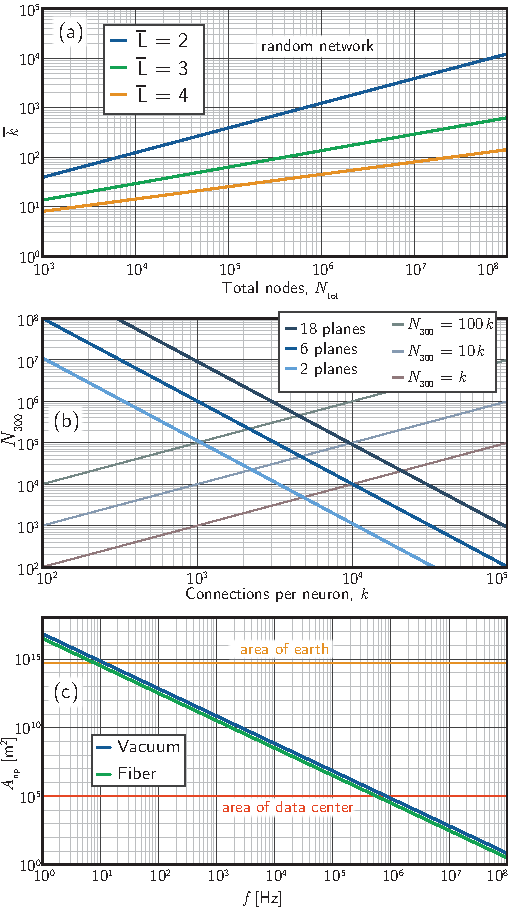
\includegraphics[width=8.6cm]{data_plots.pdf}}
	\captionof{figure}{\label{fig:data}Scaling considerations for optoelectronic neural systems. (a) The average number of connections per node required to maintain a give average path length across a random network as a function of the total number of nodes in the system. (b) The total number of nodes that can fit on a 300\,mm wafer as a function of the number of connections per node in the wire-limited regime \cite{ke1982}. (c) The area of the neuronal pool as a function of the frequency of neuronal oscillations assuming light-speed communication \cite{shICRC2018}.}
\end{figure}

\subsubsection{Clustering}
This analysis of average path length is relevant for quantifying a network's potential for information integration, but as we stated above, a neural system also depends on the ability for differentiated processing. Let us consider differentiation across various scales of the network. Ideally, no two neurons would behave identically, because this would not provide new information. Each neuron will fire preferentially in response to stimulus according to a tuning curve \cite{daab2001}. In practice, some redundancy is advantageous if a network is to rapidly gain confidence regarding the nature of a stimulus. Neural systems employ populations of neurons to represent certain pieces of information. The net activity across the population represents the presence or absence of a stimulus, and the variation in activity across the population represents uncertainty about the interpretation of the stimulus. In order for a certain population of neurons to predominantly exchange information locally and rapidly establish a consensus interpretation of a stimulus, the neurons in that population should comprise a preponderance of connections within the population. Groups of neurons with an abundance of connections within the group relative to connections external to the group form a community, and a clustering coefficient \cite{eskn2014,fa2007} is the simplest network metric. If node $a$ is connected to node $b$ and to node $c$, the clustering coefficient quantifies the fraction of cases in which node $b$ is also connected to node $c$. This metric provides insight into the tendency of neurons to form specialized communities with information processing differentiated from other parts of the network, and is first step toward analyzing the modularity of the system. 

\subsubsection{Small-World Networks}
A random network has a low clustering coefficient, as the presence or absence of a connection between nodes $b$ and $c$ is, by definition, completely independent of the presence or absence of any connections to or from node $a$. Yet the networks of the brain\textemdash from the scale of neurons to the scale of connections between regions\textemdash show a high degree of clustering relative to a random network. As we have emphasized, neural information processing relies on both differentiated processing by local clusters and efficient integration of information across the network. We therefore expect neural systems to simultaneously achieve a high clustering coefficient and short average path length. A small-world networks is one with both of these traits \cite{wast1998}. We can introduce the small-world index (SWI) \cite{hugu2008} given by  $\mathrm{SWI} = \frac{\bar{C}/\bar{L}}{\bar{C}_{\mathrm{r}}/\bar{L}_{\mathrm{r}}}$, where $\bar{C}$ is the average clustering coefficient, $\bar{L}$ is the average shortest path, and the subscript, $\mathrm{r}$, refers to a random graph. Whether analyzed at the scale of populations of a few thousand neurons or at the scale of large regions of the brain, the networks demonstrate large $\mathrm{SWI}$, indicating that different populations of neurons represent different information, the activities of these populations can be efficiently communicated across the network, and  giving hints that brain architecture is hierarchical and modular.

\subsubsection{\label{sec:modularity_and_hierarchy}Modularity and Hierarchy}
Anatomically, clusters in the brain were thoroughly described by Mountcastle in 1977 \cite{mo1978} before the concept of a small-world network had been introduced \cite{wast1998}. Mountcastle referred to the communities of neurons as mini-columns and columns. Imaging of biological neural systems with various techniques across all relevant length scales indicates modularity persists across multiple levels of hierarchy \cite{beba2017}. The clustering coefficient discussed above can be generalized to the modularity, $Q$, quantifying the degree to which the connections of a network depart from what would be expected of a random network to form partitioned communities \cite{rusp2010,beba2017}. For example, clusters of neurons are partitioned into mini-columns. At the next level of hierarchy, clusters of mini-columns are partitioned into columns. Clusters of columns are partitioned into brain regions. At the highest level of hierarchy in the brain, regions exchange information throughout the cerebral cortex and the thalamocortical complex that controls and coordinates operation of the largest modules comprising the brain \cite{bosp2015}. Neurons predominantly contribute to activity within their module, but they also must be able exchange information across partitions and up the information-processing hierarchy. Again we find differentiated, local processing combined with information integration across the hierarchical structure of the network. This neural information processing is enabled by a small-world architecture.



(probably need more here. make sure it is well set up for neuronal avalanches section and fractal use of space and time. define modular and hierarchical)

As Simon argued in 1962, `` Hierarchy...is one of the central structural schemes that the architect of complexity uses.'' \cite{si1962}. Modular and hierarchical architectures are the foundation of nearly all complex structures and systems. 

A \textbf{\textit{hierarchic system}} is ``a system that is composed of interrelated subsystems, each of the latter being, in turn, hierarchic in structure until we reach some lowest level of elementary subsystem.'' \cite{si1962}

``I shall use hierarchy in the broader sense...to refer to all complex systems analyzable into successive sets of subsystems.'' \cite{si1962}

``...we can distinguish between the interactions \textit{among} subsystems, on the one hand, and the interactions \textit{within} subsystems\textemdash i.e., among the parts of those subsystems\textemdash on the other.'' \cite{si1962}

``Empirically, a large proportion of the complex systems we observe in nature exhibit hierarchic structure. On theoretical grounds we could expect complex systems to be hierarchies in a world in which complexity had to evolve from simplicity.'' \cite{si1962} This tendency to observe hierarchical configuration in complex systems results from several factors, including the requirement of manufacturability (even in non-artificial systems such as life forms) and the efficiency resulting from the ability to optimize a small number of components and nearly independently optimize their configuration and interaction within the context of the system.

\includegraphics[width=8.6cm]{figures/_sporns_hierarchical_modularity.png}
\captionof{figure}{\label{fig:sporns_hierarchical_modularity}Schematic of a modular, hierarchical network. From Ref.\,\onlinecite{sp2010}, pg. 261.}

\includegraphics[width=8.6cm]{figures/_sporns_complexity.png}
\captionof{figure}{\label{fig:sporns_complexity}Schematic of complexity as a balance of order and disorder. From Ref.\,\onlinecite{sp2010}, pg. 282.}

\includegraphics[width=8.6cm]{figures/_sporns_complexity_and_hierarchical_modularity.png}
\captionof{figure}{\label{fig:sporns_complexity_and_hierarchical_modularity}Complexity and hierarchical modularity. From Ref.\,\onlinecite{sp2010}, pg. 291.}

\vspace{1em}
emphasize that hierarchy is defined by connections and exists even in the unform, 2D sheet of the cortex.

\subsubsection{Rentian Analysis}
%\begin{figure} 
%    \centering{\includegraphics[width=8.6cm]{rentian_analysis.pdf}}
%	\captionof{figure}{\label{fig:rentian_analysis}Caption.}
%\end{figure}
We can quantify the ability of information to be communicated up the hierarchy by analyzing the number of connections penetrating various partitions of the network, referred to as Rentian analysis. Rent's rule states that the number of edges crossing the boundary of a partition ($k$) is related to the number of nodes within the partition ($n$) by a power law of the form
\begin{equation}
\label{eq:Rent}
\varepsilon = \varepsilon_1 n^p,
\end{equation}
where $\varepsilon_1$ is the number of edges emanating from each node (first level of hierarchy), and $p$ is referred to as the Rent exponent. Rent's rule (Eq.\,\ref{eq:Rent}) was first observed in the context of VLSI circuits, and has also been shown to hold for biological neural circuits ranging from \textit{C. elegans} to the human brain \cite{bagr2010}. 

Depending on the system under study, the Rent exponent may vary, but is generally around 0.75 \cite{bagr2010}. We will demonstrate the use of Eq.\,\ref{eq:Rent} in Sec.\,\ref{sec:scaling}. The significance of the Rent exponent can be seen in its relation to the topological dimension, $D$. In Euclidean geometry, the surface area of a structure embedded in $d$-dimensional space is given by a power law of the form $s\sim v^p$. In general, the surface area $s$ scales as a length to the power of $d-1$, while the volume scales as a length to the power of $d$. Thus, in Euclidean geometry, $p = 1-1/d$, or $d = (1-p)^{-1}$. The same expression holds in fractal geometry \cite{ma1983,sc1991}, and in the case of Rentian scaling the topological dimension is related to the Rent exponent by $D = (1-p)^{-1}$, with $0 \le p \le 1$, so that $1 \le D \le \infty$. For $p > 2/3$, the topological dimension is larger than the embedding dimension, indicating that through a judicious implementation of input and output ports, information can flow through a network as if its components were connected in a higher-dimensional space. In the case of the brain, we find $D \approx 4$.

In any real network, it will only be possible to adhere to Eq.\,\ref{eq:Rent} across a certain domain of $n$. In the brain, consideration can apply from a single neuron up to the brain as a whole. Yet across this domain, Eq.\,\ref{eq:Rent} applies only piecewise, with discontinuities at certain partitions \cite{oz2004}. For example, we may expect Eq.\,\ref{eq:Rent} to hold from the scale of a single neuron up to the scale of a cortical column, but the connectivity patterns between columns are quite different than within, so we may expect a discontinuity at the scale of cortical columns, followed by a new expression of Eq.\,\ref{eq:Rent} with a different value of $p$, and perhaps a new interpretation of $n$ as the number of columns within a partition. Similarly in the domain of microelectronics, a multicore processor on a chip may obey Eq.\,\ref{eq:Rent} within each processor, with a discontinuity at the scale of the connections between processors. The wiring organization of VLSI circuits and the brain is statistically fractal, but not infinitely so. The limitations are purely physical.  

How does Rentian analysis inform our design of neural hardware? As we have emphasized, neural information is processed across a modular hierarchy. Rentian analysis quantifies the ability of information to be transmitted across partitions in the hierarchy. We conjecture that the ability for a neural system transmit more information across more levels of hierarchy will improve general intelligence. Therefore, between the neurons within a module, we expect that neural hardware should achieve high values of $D$ over a large range of $n$ before a discontinuity is necessary, so that multiple levels of hierarchy can be traversed efficiently within a module. Further, upon encountering a discontinuity, hardware must have a means of establishing another domain of Rentian scaling to efficiently collect and distribute information across more orders of hierarchy. Finally, we conjecture that the most intelligent neural hardware will provide this fractal scaling across as many levels of hierarchy as possible until the system finally reaches the limits set by the speed of communication. In Sec.\,\ref{sec:scaling} we will discuss these large-scale limits in biological and optical systems.

\subsubsection{Summary of Spatial Considerations}
The spatial structure of a neural system must comprise nodes with many edges to enable short path length across large networks. These nodes must also have high clustering to enable differentiated processing within modules. The information from these modules must be integrated across the hierarchy of the network, and the ability to do so is quantified by the topological dimension. Neural systems efficiently process information through the fractal use of space. Let us now consider their operation in time.

\subsection{Temporal Dynamics of Neural Systems}
We emphasize that neural systems make use of space and time in a coordinated manner. We have described the spatial properties of neural systems in the preceding subsection, and here we describe the temporal dynamics. In the following subsection we describe how neural systems process information across space and time to enable cognition. 

Due to the complexity of neural information processing, multiple different perspectives have emerged that emphasize different aspects of observed phenomena. These perspectives are not necessarily mutually exclusive, and a complete understanding of neural systems may require all of these concepts. This situation is analogous to the parable of the blind men and the elephant, in which several individuals attempt to understand the full nature of an elephant with access to only a subset of the relevant physical data. This analogy leads us to identify the neural elephant, depicted in Fig.\,\ref{fig:neural_elephant}. This analogy illustrates that the challenge of understanding neural information processing at the scale of the human brain is challenging enough that multiple perspectives are required to grapple with the phenomena observed to date. Here I discuss three primary perspectives that have been brought to bear on the problem. These three perspectives are: 1) oscillations and synchrony; 2) the mathematical framework of dynamical systems; and 3) neuronal avalanches and criticality. All three of these perspectives emphasize the interplay between space and time, and in Sec.\,\ref{sec:cognition} we will argue that they are all related phenomena, but like different parts of the same neural elephant.
%\begin{figure} 
%    \centering{\includegraphics[width=8.6cm]{neural_elephant.pdf}}
%	\captionof{figure}{\label{fig:neural_elephant}Caption.}
%By Hanabusa Itchō - This is a retouched picture, which means that it has been digitally altered from its original version. Modifications: rotated, cleaned, cropped, centerline fold/crease removed (original Ukiyo-e print was on two pages), and scan fog haze removed., Public Domain, https://commons.wikimedia.org/w/index.php?curid=2265247
%\end{figure}

Before exploring these three perspectives on dynamical activity in neural systems, it is necessary to review basic behaviors at the device level. In the next subsection we describe neuronal device dynamics, including relaxation oscillations, neuronal communication mechanisms, synaptic plasticity mechanisms, and computations performed by synapses and dendrites. 

\subsubsection{Device Dynamics}
A neuron is a dynamical entity. It receives input from many afferent synapses, identifies coincidences and sequences between the activities on multiple synapses, and integrates various inputs over time. In a biological neuron, activity on a synapse results in a post-synaptic current into the receiving neuron. This current reduces the magnitude of the voltage across the neuron's cell membrane, usually with an exponential decay in time, and if that voltage is reduced below a threshold, the neuron produces an action potential, often referred to as a spike or pulse. This dynamical process of signal accumulation followed by bursting activity qualifies a neuron to be considered a relaxation oscillator. Before describing the temporal dynamics of neural systems in more detail, let us consider for a moment why relaxation oscillators are particularly well suited for cognition.

\paragraph{Relaxation Oscillators}
As we have mentioned, a defining aspect of cognitive systems is the ability to differentiate locally to create many sub-processors, but also to integrate the information from many small regions into a cohesive system, and to repeat this architecture across scales. A network of many dynamical nodes, each with the capability of operating at many frequencies, gives rise to a vast state space. As computational primitives that can enable such a dynamical system, oscillators are ideal candidates. In particular, relaxation oscillators \cite{st2015,mist1990,soko1993,lued1997,huya2000,bu2006,gile2011,vepe1968,cacl1981} with temporal dynamics on multiple time scales \cite{soko1993} have many attractive properties for neural computing, which is likely why the brain is constructed of such devices \cite{ll1988}. We define a relaxation oscillator as an element, circuit, or system that produces rapid surges of a physical quantity or signal as the result of a cycle of accumulation and discharge. Relaxation oscillators are energy efficient in that they generally experience a long quiescent period followed by a short burst of activity. Timing between these short pulses can be precisely defined and detected \cite{bu2006}. Relaxation oscillators can operate at many frequencies \cite{huya2000,more} and engage with myriad dynamical interactions \cite{lued1997}. The oscillator's response is tunable \cite{huya2000}, they are resilient to noise because their signals are effectively digital \cite{stgo2005}, and they can encode information in their mean oscillation frequency as well as in higher-order timing correlations \cite{pasc1999,thde2001,sase2001,stse2007,brcl2010,haah2015}.

\paragraph{Information Coding by Relaxation Oscillators}
The spiking nature of relaxation oscillators enables them to encode information in several ways. Most simply, they can encode information in their average firing rate, which gives rise to the standard expression used in deep learning and neural networks:
\begin{equation}
\label{eq:standard_neural_network_activation} 
y_i = f(\sum_{ij}w_{ij}y_j),
\end{equation}
where $y_i$ represents the ``activation'' of the $i$th neuron, $w_{ij}$ is the synaptic weight from neuron $j$ to neuron $i$, and $f(\cdot)$ is a nonlinear function representing the input-rate-to-output-rate transfer function of a simple point neuron. Equation \ref{eq:standard_neural_network_activation} is an extremely simple model of a neuron in the sense that only the average firing rate is considered, so no information regarding the precise times of spikes is retained. Further, $w_{ij}$ is assumed to be independent of frequency, so the model assumes synapses and dendrites perform no spectral filtering. Also, all input synapses are assumed to terminate on a single integrating body, assumed to be the soma, so no information regarding the spatial location of the synapse on the dendritic tree is retained. Nevertheless, Eq.\,\ref{eq:standard_neural_network_activation} has proven remarkably useful as a starting point for deep learning. 

Beyond the rate-coded, point neuron model, relaxation oscillators can also encode information through several other means. These include the time-to-first-spike after the onset of a stimulus, the phase of a spike relative to sinusoidal background oscillations, and the time interval between the firings of two or more neurons (see Sec. 4.5 in Ref.\,\cite{geki2002}). Thus, while information coding in digital computing is simple (bits are transmitted one at a time on a clock), information processing in neural systems with relaxation oscillators as computational primitives is complex. Neurons and networks do not speak a single, simple language, but rather send various types of spike-based messages with different information encoding and decoding in different contexts. We will explore these various strategies for coding in more detail shortly, but first we note one simplifying factor: the spikes that are used to communicate between neurons are binary. No information is conveyed in the amplitude of a single spike.

\paragraph{Binary communication and post-synaptic response}
We expect that any cognitive computing platform will be based on spiking neurons that behave as relaxation oscillators. Communication between these relaxation oscillators is effectively binary\textemdash all or nothing. When a neuron produces an action potential, it propagates down the axon and branches throughout the axonal arbor. The signal propagates as a section of depolarization between the interior of the axon and the surrounding extracellular fluid. This depolarization opens pores in the membrane of the axon, allowing the flow of ions from the extracellular fluid into the axon, thus providing the electrical signal that will reach the synapses. Each time the action potential is generated, the behavior is nearly identical: the speed of propagation of the signal is set by the physical properties of the axon; the number of pores that open is very large, so the signal propagating down the axon is not noisy; and the signal that reaches the synapses is very similar from pulse to pulse. Significant variability arises when an action potential meets a synapse, but this relates to the information processing occurring at the synapse (discussed in more detail below), not the nature of the encoding of the signal. 

To realize the digital nature of neuronal communication, the role of the action potential propagating down the axon is not to provide current to the post-synaptic neuron, but rather to begin a chemical cascade within the synapse that controls the post-synaptic signal amplitude. When the action potential reaches the synapse (pre-synaptic cleft), the action potential may trigger the release of neurotransmitters into the synaptic cleft. These neurotransmitters diffuse through the fluid of the cleft, and bind to receptors on the post-synaptic cleft. These receptors then trigger the flow of current through the dendrite on which the synapse resides. This post-synaptic current carries the information that will be processed, first by the dendrite, then the dendritic tree, and finally the soma. The action potential arriving at the synapse initiates the synaptic cascade in a binary, all-or-nothing manner (either vesicles are released from the pre-synaptic cleft or they are not), but the amount of current flowing into the post-synaptic dendrite depends on the state of the synapse, and it can take a continuum of values. Thus, communication in neural systems is binary, yet information processing is analog. The synapse performs a digital-to-analog conversion, and the state of the synapse (which depends on many factors) determines the analog value entering into the computation performed by the dendrites and soma. 

When a synapse receives an action potential, it has a certain probability of releasing vesicles containing neurotransmitters that will then be detected on the receptors of the post-synaptic cleft, generating a current that will propagate a certain distance and decay with a certain time constant. The time-course of the response is a continuous function, specifically an exponential decaying in space and time. The length and time constants depend on: the type of synapse; the morphology of the dendrite to which it is connected; the concentration of various neuromodulators; and the local membrane potential, which is determined by local synaptic activity. Thus, communication between neurons is well modeled by binary events that trigger a post-synaptic current with some probability $P_{\mathrm{s}}$, while the post-synaptic current is highly variable and shaped by a number of physiological and dynamical factors. We will further explore the relevance of this post-synaptic response in the coming paragraphs. 

\paragraph{The Neuron as a Complex Information Processing System}
For multiple reasons described above, we expect relaxation oscillators to be the computational primitives of complex cognitive systems. But amongst relaxation oscillators, neurons are unique in the myriad complexities. Our understanding of the information-processing capabilities of neurons has evolved considerably over time. Early models treated a neuron as a point that passively integrated many inputs and produced a signal upon reaching threshold. This integrate-and-fire model was proposed as early as 1906 by Sherrington in a series of lectures \cite{sh1906}, supporting the view championed by Ram\'{o}n y Cajal \cite{ra1908}. It was that same year that Ram\'{o}n y Cajal shared the Nobel Prize in Physiology or Medicine with Golgi for their work on the structure of the nervous system. Within this point-neuron view, a neuron simply integrates signals over time, so information regarding the timing or location of synaptic activity is lost. Further, the complex, dendritic tree is assumed to passively transmit synaptic signals to the neuron cell body. 

This view of the neuron as a point integrator was highly influential, and remains the dominant model guiding many efforts in deep learning and even neuromorphic hardware. However, further experimental evidence as well as theoretical arguments have deepened our understanding of how neurons work and led to a picture of neural information processing that is far more subtle and powerful. 

The modern picture of neural information processing reveals that many operations in addition to integration are being performed, and that these computations are performed at synapses, through the dendritic tree, and in the neuron as a whole. Some of the additional operations now believed to be performed by neurons include: coincidence and sequence detection; nonlinear thresholding performed in dendrites; temporal filtering of pulse trains; and bursting to overcome noise and enable selective communication between subsets of neurons in an ensemble. We now review each of these concepts and explain their significance for neural information processing.

\paragraph{Coincidence and Sequence Detection in Active Dendrites}
As discussed above, after a synapse is triggered and a post-synaptic response is induced, the time-course of the post-synaptic response is a decaying exponential with a time constant that can be shaped by a number of factors. Whether a neuron simply integrates signals or detects coincidences depends on this time constant of the post-synaptic potential relative to the average neuronal interspike interval. If the time constant is on the order of the interspike interval of the neuron, temporal integration is performed during the entire interspike interval, and the neuron is well-modeled as an integrator. If the time constant is short compared to the interspike interval, neurons perform coincidence detection, meaning only spikes that are coincident on the neuron within a short time window relative to the interspike interval can induce the neuron to produce an action potential. If integration is performed exclusively, then the timing of spikes conveys no information. If coincidence detection occurs, information is conveyed in spike timing, neurons respond preferentially to synchronized inputs, and a neuron's output reflects the input pattern.

Work in the 1990s led K\"{o}nig, Engel, and Singer to argue that cortical neurons are better modeled as coincidence detectors than integrators \cite{koen1996}. Their arguments were based both on the physiological evidence that many synapses can have time constants much shorter than the average interspike interval as well as theoretical arguments related to information processing. Regarding the latter, multiple benefits can be identified \cite{sase2000,sase2001}. First, speed of response can be improved if coincidences can be utilized. Processing speed is determined by the latency between the time of arrival of a signal and the time of a generated response. As stated in Ref.\,\onlinecite{koen1996}, ``Because only a small subset of all afferent [post-synaptic potentials] are relevant (namely those which actually conicide and trigger an action potential), the mean time-lag between relevant input and output signals is very short\textemdash only a fraction of the interspike interval. Thus, at identical interspike intervals neuronal systems utilizing coincidence detection can process information much faster.'' Second, coincidence detection provides benefits with regard to error propagation and noise. Errors due to stochastic processes in the environment are effectively filtered out by coincidence detection, as they would only contribute to neuronal firing rarely when they coincide with true signal, whereas neurons performing integration sum all incoming activity uniformly, regardless of correlations that may serve to isolate signal from noise. Third, the use of coincidence detection allows neural systems to make use of smaller ensembles of neurons for encoding information, referred to as the size of the `grain' in Ref.\,\onlinecite{koen1996}. If coincidences give rise to larger post-synaptic signals, then synchronized activity of a small group of neurons can have a large effect and drive a neuron to spike. Finally, the main strength of coincidence detection temporal information is not discarded, and synchronized inputs are processed differently than asynchronized inputs on the same set of synapses. The ability to respond preferentially to synchronized inputs has important consequences for information integration and binding, as discussed below in Sec.\,\ref{sec:oscillations_and_synchrony}. If neurons can detect coincidences, several important computation become possible. 

Work elucidating the behavior of dendrites further supports the view that neurons make use of the timing of synaptic activity as well as other intricacies beyond simple integration \cite{stsp2015}. As stated by Koch in 1997, ``...dendrites do much more than simply convey synaptic inputs to the cell for linear summation. Indeed, if this were all they did, it is not obvious why dendrites would be needed at all; neurons could be spherical in shape and large enough to accommodate all the synaptic inputs directly onto their cell bodies. ...the function of this elaborate structure cannot simply be to maximize the surface area for synaptic contact.'' \cite{ko1997} Instead of acting as passive transmission lines, the active properties of dendrites \cite{joma1996} give rise to the ability to detect coincidences. The basic mechanism relies on the nonlinearity of the response of a dendrite. If two synapses are located in close proximity on a dendrite, the response of the dendrite is a nonlinear function of the activities of the two synapses. Whereas the response of a passive dendrite would be the sum of the activities of the two synapses, the true dendritic response is closer to the product of the activities of the two synapses \cite{ko1997}. Further, dendrites themselves can generate spikes upon reaching threshold \cite{hoko2006}, a behavior once thought only to occur in the neuron as a whole. Again considering the example of two synapses on a dendrite, if only one of the synapses fires within the decay time of the post-synaptic potential, it may be insufficient to generate a dendritic spike, and the neuron is not informed of the synaptic activity. However, if both synapses fire within the decay time it may be sufficient to induce a dendritic spike, and the information is passed along the dendritic tree toward the soma. By 2006, the physiological mechanisms of dendritic spikes were more clearly understood \cite{hoko2006}, providing the device-level mechanism to support the coincidence-based information processing described by K\"{o}nig, Engel, and Singer in 1996. The nonlinear response of a dendrite with two synapses can also be compared to a logical AND operation: if synapse one AND synapse two fire within a certain time window, an output pulse is produced. 

The processing capabilities of dendrites extend beyond detection of coincidences between two synapses. Consider now $n$ synapses connected to a single dendrite. Now the dendrite will perform a nonlinear function on the inputs of the $n$ synapses, leading to an intermediate nonlinear transfer function between the synapses and the neuron as a whole. A neuron comprising many such dendrites will behave as a complex processor comprising multiple independent threshold units, and giving rise to myriad different transfer functions depending upon precisely which afferent synapses are active at a given time, just as observed in recent experiments \cite{sava2017}. Further, due to the morphology of a given dendrite, the post-synaptic current will often flow in a particular direction, usually toward the cell body. Consider the case where synapse one makes contact furthest from the cell body and synapse $n$ makes contact closest to the cell body. In this case, firing of synapse one will lead to a post-synaptic current that flows toward synapse two, thereby lowering the local membrane potential at synapse two. If a synaptic firing event at synapse one is followed closely by a firing event at synapse two, dendritic current is more likely to propagate on to synapse three, thereby lowering the membrane potential there. The pattern extend to synapse $n$, and this nonlinear signal propagation along the dendrite provides a means for the dendrite to detect specific sequences of activity: if synapse one fires just before synapse two, and synapse two is just before three, etc., then the dendrite is far more likely to produce a spike that propagates to the cell body than if the synapses fired in a different order. This phenomenon is illustrated schematically in Fig.\,\ref{fig:dendritic_sequence_detection}. The ability of neurons to make use of such sequence detection was developed in 2016 by Hawkins and Ahmad \cite{haah2015}. (say a bit more here) Interestingly, humans appear to be the species with the most elaborate dendritic trees \cite{el2003}.

\vspace{3em}
The total potential generated along a dendrite ``depends therefore on the temporal order of the stimulation of the synapses. An input sequence starting at the far end of the dendrite and approaching the soma is more effective in triggering an output spike than the same number of input spikes in reverse order.'' (\cite{geki2002}, pg. 144.)

%\begin{figure} 
%    \centering{\includegraphics[width=8.6cm]{dendritic_sequence_detection.pdf}}
%	\captionof{figure}{\label{fig:dendritic_sequence_detection}Caption.}
%\end{figure}

I will discuss dendrites further in the context of learning and plasticity shortly. First I review work related to communication between neurons through bursting.

\vspace{3em}
For detection of temporal information in the brain, cite review article from 1993 \cite{ca1993}. You have not read this article, so be careful.

\paragraph{Communication in Bursts}
If neurons encoded information only in their average firing rate, we would expect most neurons to fire relatively consistently, with the exact value of the rate dynamically varying depending on stimulus. By contrast, if neurons encoded information only in spike timing and coincidences, we would expect them to fire single action potentials when presented with relevant stimuli. In practice, these two behaviors are both observed, but a more common mode of activity is the burst. A neuronal burst is a closely spaced sequence of spikes followed by a long quiescent period. 

%bursting for reliability
Bursting activity is thought to play a central role in communication between neurons, perhaps as important as rate or other forms of temporal coding. One function of communication via bursts was appreciated by the 1990s, and that is the increased reliability of communicating with bursts rather than single spikes \cite{li1997}. A single synapse can be unreliable at producing a post-synaptic current in response to the arrival of a single action potential. On the device level, this is because vesicle release by the pre-synaptic cleft does not occur deterministically, but rather with probability $P_{\mathrm{s}}$, which varies considerably across synapses, and can be less than 0.1. However, the arrival of a number of action potentials in close succession performs a facilitating function that increases the probability of vesicle release with the arrival of each successive pulse. While the synaptic response to a single action potential can be unreliable, the response to a burst is much more reliable, increasing $P_{\mathrm{s}}$ above 0.9 simply by using two pulses instead of one in some observations \cite{fomc1991,degu1996}, a phenomenon known as paired-pulse facilitation \cite{li1997}. 

This reasoning of bursts being more reliable than single spikes is intuitive, but it may lead one to suspect that bursts effectively make communication analog in the sense that the generated post-synaptic current will depend on the number of spikes in the burst. Lisman has argued based on physiological evidence that this is not the case. The nuances of vesicle release and neurotransmitter detection are such that the post-synaptic current is nearly identical when receiving a burst, independent of the number of spikes in the burst (within a workable range) \cite{li1997}, thereby enabling bursting to overcome synaptic failure while maintaining binary communication.

Within this picture of neuronal bursting, the low probability of synaptic response becomes advantageous for filtering noise. As Lisman argues, in some brain regions, single spikes are simply the result of noise, but bursts are rarely noise. Therefore, if a synapse responds only to bursts of two or more pulses, it effectively ignores the noise, and responds only to the signal. For example, place cells in the hippocampus \cite{frbu2018} fire preferentially when the organism is in a specific location for which that neuron's tuning curve is maximized. It has been shown that responding only to bursts can define the place field more accurately than when single spikes are considered \cite{otei1991}. Similarly in visual cortex, it is well-known that neurons can have a tuning curve maximized to detect gratings with a specific spatial frequency or orientation \cite{daab2001}. It has been shown that only the bursting component of a neuron's activity is tuned to represent these quantities, while isolated spiking activity only correlates with the contrast of the light and dark regions of the grating \cite{cama1981}. These ideas lead Lisman to conclude ``that the ability of synapses to not transmit single spikes might be a crucial form of filtering.'' \cite{li1997} 

%bursting for frequency-selective communication
The concept that neurons fire in bursts to overcome unreliable synapses and filter noise is well supported by theoretical and experimental evidence. Yet these may not be the only reasons for communication in bursts. Izhikevich et al. have argued another principle is also in play: ``bursts with specific resonant interspike frequencies are more likely to cause a postsynaptic cell to fire than are bursts with higher or lower frequencies. '' \cite{izde2003} Within this model, neurons firing in bursts are like radio transmitters, and some synapses are tuned to receive spike trains of the same frequency. This tuning of synaptic and neuronal responses can be achieved through a combination of high- and low-pass filtering as well as subthreshold oscillations of the membrane potential. These device mechanisms for frequency selectivity are discussed below in Secs.\,\ref{sec:short_term_plasticity} and \ref{sec:subthreshold_membrane_oscillations}. 

The most exciting aspect of this use of bursting is that ``the same burst could resonate for some synapses or cells and not resonate for others,'' thereby providing ``effective mechanisms for selective communication between neurons.'' Such a method of targeted communication is one of many examples of how neurons can utilize one vast structural network to enable myriad functional networks at different times in different contexts. Izhikevich et al. argue that communication via bursts enables targeted, resonant communication \textit{in addition} to making communication more reliable and filtering noise. Beyond these motivations related to improvements in communication, bursts may also be more effective at modifying synaptic efficacy. I discuss the role of bursting in long-term synaptic modification below in Sec.\,\ref{sec:long_term_plasticity}.

\paragraph{\label{sec:coding_strategies_summary}Summary of Coding Strategies}
We have discussed rate coding, coincidence detection, sequence detection, and bursting. One may ask the question, ``Which of these is actually used by the brain?'' The answer is all of them. In some contexts, the average firing rate of a neuron may represent the content of a stimulus. In other contexts, the precise timing between two synaptic events or the order in which multiple synapse events occurs carries information that is utilized by the receiving neuron. In still other contexts, bursts are used to increase reliability, filter noise, and the frequency of pulses within a burst can enable selective communication between resonant elements of the network. All of these coding strategies and communication mechanisms contribute to the extraordinary efficiency and adaptability of biological neural systems, and we should aspire to incorporate all of these principles in the design of hardware for general intelligence. 

We now summarize the mechanisms at the device level that enable these subtle and sophisticated mechanisms for information processing.

\paragraph{\label{sec:short_term_plasticity}Short-Term Synaptic Plasticity}
As described above, the ability of a synapse to respond preferentially to activity at a specific frequency enables additional complexities in communication. At the device level, frequency-selective synaptic response is enabled by filtering mechanisms referred to as short-term synaptic plasticity. 
%Fig. 1 of \cite{izde2003}
%\begin{figure} 
%    \centering{\includegraphics[width=8.6cm]{short-term_plasticity.pdf}}
%	\captionof{figure}{\label{fig:short-term_plasticity}Caption.}
%\end{figure}
The state of a synapse is affected by its activity over short and long time scales as well as external network factors. Neurons often signal in bursts (closely spaced sequences of spikes) \cite{iz2007}, and within a burst, the time between spikes is referred to as the inter-spike interval. Changes of synaptic response over time scales on the order of the inter-spike interval are referred to as short-term synaptic plasticity \cite{abre2004}. One key effect of short-term plasticity is to perform a temporal filter on an afferent spike train. This can be a high-pass, low-pass, or band-pass filter, as shown in Fig.\,\ref{fig:short-term_plasticity}. High-pass filtering results in only the first few pulses of a train being transmitted from the pre-synaptic axon to the post-synaptic dendrite. A synapse performing high-pass filtering reports to the post-synaptic neuron that the pre-synaptic neuron has begun to fire. Conversely, low-pass filtering results in synaptic response after the first several pulses of a train have occurred. A synapse performing low-pass filtering will not be active unless the pre-synaptic neuron produces a pulse train of a certain minimum duration, and therefore this synapse reports to the post-synaptic neuron when the pre-synaptic neuron has sustained bursting activity beyond a certain duration. Band-pass filtering combines these responses. A synapse performing band-pass filtering will only produce a response after an afferent pulse train exceeds a certain duration, and it will fall silent again after if the afferent pulse train continues beyond a certain duration.

These short-term filtering mechanisms enable synapses to report much more information to the neuron than simply the time-averaged rate of afferent activity. A neuron combining the signals from many synapses with various short-term responses has access to information regarding not just the average spike rates of the neurons from which it receives synaptic connections, but also regarding the initialization of bursting and the duration of spike trains.


\paragraph{\label{sec:subthreshold_membrane_oscillations}Subthreshold Membrane Oscillations}

\paragraph{\label{sec:long_term_plasticity}Long-Term Synaptic Plasticity}
%\begin{figure} 
%    \centering{\includegraphics[width=8.6cm]{stdp.pdf}}
%	\captionof{figure}{\label{fig:stdp}Caption.}
%\end{figure}
Over time periods much longer than the inter-spike interval, the response of synapses can also change based on the activity of the two neurons involved in the synapse. A synapse that is more active will strengthen (long-term potentiation), and a synapse that is used less will weaken (long-term depression). This was the essential insight of Hebb in 1949 \cite{he1949}, a concept that developed in the subsequent decades \cite{bipo1998,somi2000} to account for the fact that long-term potentiation only occurs if the pre-synaptic neuron fires just before the post-synaptic neuron, indicating the potential for causality, while long-term depression is induced when the pre-synaptic neuron fires just after the post-synaptic neuron. This spike-timing-dependent plasticity (STDP) \cite{mage2012} plays a central role in memory formation and network adaptation. 

The physical mechanism responsible for STDP involves the growth and decay of neurotransmitter sources and receptors present at the synapse. These synaptic molecular machines (N-methyl-D-aspartate receptors, NMDARs) develop in response to the action potential arriving at the pre-synaptic terminal as well as the back-propagating signal from the post-synaptic neuron. The complex chemistry present at each synapse leads to a remarkable degree of diversity and adaptability in synaptic response.

By strengthening cooperative synapses, STDP adapts the structural network of neurons and their connections into functional networks embodying certain memories or computations learned over time based on the correlations of neuronal firing events. It has been shown that random networks with synaptic weights adjusted over time by STDP adapt into small-world networks \cite{shki2006}, maintaining efficient communication, and adding functional clusters specialized for specific computations. This is one example of the structural network of a neural system can be used to manifest multiple functional networks.

The functional clusters established via STDP have spectral signatures. A given functional cluster of neurons will have a specific pattern of activity, that may repeat in time. The period of this repetition will depend on the specific parameters of the circuit, and a large structural network comprising many highly connected neurons will have the potential to establish a vast repertoire of functional clusters with oscillations at many frequencies. Through STDP, the network can increase the activity of certain oscillations corresponding to highly utilized functional modules. If a certain stimulus has a probability of activating a certain functional cluster, the overtime, the action of STDP will enable the network to correlate that stimulus with the dynamical response of the cluster, and the stimulus will evoke the activity of the cluster with higher probability. In the language of dynamical systems, a specific cyclical response of the functional cluster is referred to as a basin of attraction \cite{iz2007,st2015}, and STDP ensures that relevant stimuli lead the network to the appropriate basin of attraction. This is function of an autoassociator, and it is an important form of long-term memory (\cite{bu2006} pg. 329).

Spike-timing-dependent plasticity makes use of correlations between firing activity of neurons to adapt the network into functional clusters \cite{shki2006}, store memories in dynamical sequences \cite{haah2015}, and strengthen circuits that demonstrate temporal patterns storing sequential memories (\cite{bu2006} pg. 318). But theoretical analysis finds that if STDP is the only long-term synaptic plasticity mechanism, memories are forgotten very quickly \cite{fuab2007}. Experimental analysis finds that synapses have multiple additional means to change how synapses adapt over time and activity to help retain memories \cite{ab2008}. These plasticity mechanisms are referred to collectively as metaplasticity.

%bursting for plasticity
It has been shown that a burst of action potentials comprising four pulses can be sufficient to induce long-term potentiation and depression \cite{huli1995}, dependent on the timing of the burst relative to theta oscillations. A burst arriving at the peak of theta leads to potentiation, while a burst arriving at the trough leads to depression. In this case, we find an interplay between neuronal bursting, synchronized oscillations, and synaptic plasticity. Adapting based on the confluence of all this information leads to efficient evolution toward a network structure that generates constructive activity.

\paragraph{Metaplasticity}
While STDP adapts the strength of synapses (synaptic efficacy), metaplasticity adapts the rate at which synaptic efficacy changes over time and activity. For example, if a pre-synaptic neuron fires just before a post-synaptic neuron, the synapse connecting the two will be a candidate to experience long-term potentiation. But the \textit{probability} that the synapse actually does potentiate can be controlled by chemical signals within the synapse. Additionally, the \textit{amount} by which the synaptic efficacy changes is also subject to chemical modulation. 

The function of metaplasticity is to control which neural circuits adapt at a given time \cite{ab2008}. The receptors mentioned above (NMDARs) can be controlled based on a variety of factors related to network activity so that adaptability may be turned on and off in certain regions at certain times. This functionality is required of plastic synapses to keep them from too quickly losing the trace of a memory that is still needed. Experiments with humans indicate that forgetting occurs as a power-law function of time, \cite{wieb1991,wieb1997}, yet Fusi and Abbott have shown that memories are lost more rapidly than this if plastic synapses are presented with continual stimulus \cite{fuab2007}. They have proposed a model that achieves the observed power-law forgetting by introducing internal complexity to the synapses \cite{fudr2005}. In this model, each synapse has various states of efficacy (weak and strong synaptic weight), but it also has additional internal states with the same efficacy. The difference between these states is the probability with which the efficacy will change due to future plasticity events. 

Metaplasticity provides a network with the means to to enable some regions to adapt at a given time, under a given stimulus, while other regions are unchanged at that time, under that stimulus. Further, metaplasticity provides a means by which some synapses within a region may change very rapidly to adapt to a new stimulus, while other synapses in the same region may change slowly or not at all when presented with the same stimulus. We expect that an intelligent neural system have the capability to immediately learn in response to new information, but also to maintain a lasting representation of all that has been learned through the network's existence even in the presence of continually varying input. Metaplasticity is an important means by which rapid learning in conjunction with long memory retention can be achieved. As stated by Abraham, ``...these metaplasticity processes represent a major form of adaptation that helps to keep synaptic efficacy within a dynamic range and larger neural networks in the appropriate state for learning.''

\paragraph{Homeostatic Plasticity}
To conclude this discussion of synaptic plasticity mechanisms, we note that short-term plasticity adapts based only on the activity of the pre-synaptic neuron, while STDP adapts based on correlations in the activity between pre- and post-synaptic neurons. The mechanism of homeostatic plasticity \cite{cube2012} adapts synaptic weights based only on the activity of the post-synaptic neuron. Homeostatic plasticity (also referred to as the Bienenstock-Cooper-Munro (BCM) model \cite{bico1982}) adjusts the synaptic weights of synapses incident upon a given neuron based on a sliding temporal average of the recent firing activity of that neuron. Such a mechanism provides a means by which neuron and network activity can be maintained within useful limits and dynamic range can be maximized.

\paragraph{\label{sec:dendritic_processing}Dendritic Processing}
We have discussed how STDP leads to the formation of functional clusters within a network based on the history of correlated neuronal activity. But what if the network wishes to isolate specific functional clusters on time scales as short as an inter-spike interval? Or what if we wish to endow a neuron with the ability to respond not only to activity in single synapses, but rather to integrated activity from specific clusters of synapses, or to specific sequences of activity within a cluster of synapses? Dendritic processing enables these functions.

Dendritic processing refers to the intermediate, nonlinear transfer functions performed by dendrites between individual synapses and the neuron as a whole \cite{stsp2015}. The dendritic arbor is a complex, branching structure on which most of a neurons input synapses make their connections. While the dendritic tree was thought to be a passive integrating structure for quite some time, by the mid 1990s many activite dendritic responses were beginning to be understood \cite{joma1996}. The dendritic branches that comprise the arbor have passive and active properties that allow them to perform various computations. Dendrites modulate postsynaptic potentials on their way to the soma as well as generate spike activity \cite{majo2005,hoko2006}. One picture of the dendritic arbor is a network of multiple independent threshold units that integrate signals and produce dendritic spikes upon reaching threshold. This picture was introduced on theoretical grounds based on the enhanced storage capacity of such a dendritic tree in 2001 \cite{pome2001}, and supporting experimental evidence continues to accure \cite{sava2017}.

For example, consider a dendrite with two synapses. If the post-synaptic current into the dendrite is sufficient to produce a dendritic spike, and if this dendritic spike has the same form whether one or both synapses fire, the dendrite performs the OR operation. If both synapses are required to fire to produce a dendritic spike, it performs the AND operation. The current generated in a dendritic spike propagates only a short distance along the dendritic tree, into the next dendritic compartment closer to the cell body, and the current decays with an exponential time constant. Thus, dendrites can perform basic logical operations with a temporal component, and activity closer to the base of the dendritic tree at the cell body integrates information from a larger number of inputs. 

Like many aspects of neural information processing, the myriad roles of dendrites remind us that the devices giving rise to cognition are diverse and multifunctional. Mel, Schiller, and Poirazi emphasize that ``dendrites of different neuron types contribute to the cell's input-output function in markedly different ways.'' \cite{mesc2017} While all of the aforementioned roles of dendrites are observed in biological neural systems, they are not necessarily all present in every dendrite. In the context of designing hardware for neural information processing, these functions must be available, and sophisticated analysis at the level of networks and systems must inform our decisions of when to include each mechanism.

\cite{pome2001}


\paragraph{\label{sec:dendrites_and_plasticity}Dendrites and Plasticity}
In addition to performing nonlinear transfer functions on inputs, dendrites also play a key role in synaptic update and learning. This activity is induced by back-propagating action potentials created during the firing of the neuron \cite{majo2005}. These back-propagating action potentials provide a feedback signal from the neuron to the dendrites and synapses after neuronal firing that performs one of the steps in a timing-dependent plasticity process \cite{nesa2004}.

In addition to back-propagating action potentials playing a role in STDP, dendritic spikes are also involved in forms of synaptic plasticity that do not require synaptic activity. In these forms of synaptic plasticity, it is the timing of the forward-propagating dendritic spikes and backward-propagating spikes that establish the conditions in which synaptic weights can be modified \cite{hoko2004}. This local activity can lead to long-term synaptic potentiation or depression and may be the primary mechanism for rapidly acquiring memories \cite{hoko2006}.

We have mentioned that dendrites are capable of acting as integrators or coincidence detectors depending on the time constants involved. Additionally, a single dendrite can transition between these two roles based on the interplay between synaptic activity and the neuromodulatory environment \cite{hoko2006}. The presence of certain neuromodulators affects the behavior of voltage-gated ion channels, thereby shaping the short-term response of dendrites \cite{majo2005}. As stated by Holthoff et al., ``...the alliance of non-linear and linear integration modes combines the advantages of the excellent signal-to-noise ratio of digital processing with teh speed and complexity of analog processing.'' \cite{hoko2006} 

We have also mentioned that back-propagating action potentials in dendrites play a central role in STDP. The active properties of dendrites can lead to metaplasticity as well \cite{ab2008}. The mechanisms involved again relate to the interactions between synaptic inputs and neuromodulators. The interplay between neuromodulators and synaptic activity affects the time constants that shape the dendritic membrane potential as well as the probability that potentiation or depression will occur in the presence of synaptic input. 

This discussion of dendritic processing is necessarily brief, emphasizing the active role played by dendrites in adaptive and frequency-selective response to spike trains based on voltage-dependent conductances; the nonlinear thresholding properties of dendrites exemplified by the generation of dendritic spikes; and the role of the dendritic tree and back-propagating action potentials in synaptic plasticity. Further detail can be found in the comprehensive review by Sj\"{o}str\"{o}m et al. \cite{sjra2008} From a computational perspective, the dendritic tree is the main information-processing infrastructure of a neuron. Computations are performed as fan-in occurs. Whereas in many computational systems, fan-in is passive and represents part of the communication infrastructure, in neural systems fan-in and computation occur in the same physical structures. This is in contrast with the axonal arbor, which performs fan-out to many synapses, but the axons themselves do not modify information, but rather simply serve to communicate spikes from one neuron to many others. 

\paragraph{Summary of Neural Device Dynamics}
This subsection summarized literature supporting the perspective that relaxation oscillators are uniquely suited to serve as computational primitives in cognitive systems due to the high signal-to-noise ratio of their outputs, their adaptive frequency response, and their ability to make use of many information coding schemes. These coding schemes have been described. The importance of binary communication for mitigating noise was discussed, and multiple communication schemes were explained. These modes of communication include: average rate; coincidence and sequence; phase relative to background oscillations; and bursting for reliability as well as frequency selectivity. The device-level mechanisms that enable these functions were summarized, including short- and long-term synaptic plasticity and active dendritic functions. We now turn our attention to activity emerging from populations of neurons.

\subsubsection{\label{sec:populations}From devices to populations}
We have described some of the basic device operations of neurons and their components, but neural information processing leverages entire populations of neurons with emergent mechanisms for information processing occurring in a network context. As a first example, consider a population of uncorrelated, non-interacting neurons receiving identical stimulus and firing asynchronously. The population activity is defined as the sum over all firings by all neurons, and in the presence of a constant stimulus, the population will fire with a fixed population activity. For a large population of $N\longrightarrow\infty$ neurons, at a given moment there will be some neurons  at all stages of the cycle of integration and firing. If the stimulus is instantaneously increased by a finite amount (perhaps due to the input from another neuron firing), the population activity will instantaneously increase. This instantaneous response is possible because some neurons in the population will be close to threshold, and the finite perturbation pushes them over threshold. Thus, they fire sooner than they would have in the absence of the perturbation, and the population activity increases. Such a response is not obtained, in general, from a single neuron. If a single neuron is perturbed instantaneously, its response will depend on its state before the perturbation. If it is in a refractory period or far from threshold, the perturbation may be insufficient to evoke a response at all, or it may take some time before the effect of the perturbation is observed.

This rapid population response is most clearly observable in the absence of noise, and in the presence of noise, populations perform useful functions as well. For example, one can calculate the signal-to-noise (SNR) ratio of a group of neurons attempting to code a given signal. It is found the SNR increases linearly with the number of neurons in the population (\cite{geki2002}, chapter 7.3.2). Populations of neurons can increase response time and mitigate noise. These two responses do not require interactions between the neurons in the population, yet dynamics become more interesting when the neurons of a population are connected with various graph structures.

\paragraph{\label{sec:oscillations_and_synchrony}Oscillations and synchrony}
When observing brain activity at a coarse scale, such as with electroencephalograms, sinusoidal oscillations in activity are observed. Finer measurements with electrodes also observe this phenomenon on shorter length scales. Oscillations in mammalian cortical neurons are observed across five orders of magnitude in frequency, from 0.05\,Hz to 500\,Hz \cite{budr2004}, and the types of oscillations observed depend on behavior and input stimulus. In rats, 10 frequency bands are observed, and their center frequencies are separated logarithmically, creating what Buzs\'{a}ki refers to as ``a system of brain oscillators''. These different bands are associated with different brain states and different behaviors. At a given moment, activity may be present in several frequency bands, and these activities may compete or interact with each other.   This seemingly simple behavior leads to many layers of complexity with important ramifications for neural system operation \cite{bu2006}. Each neuron is a relaxation oscillator, characterized by spikes that are short in time relative to the inter-spike interval. A single neuron is not well modeled by a sinusoidal time dependence, but the net activity of a population of neurons often takes a sinusoidal form. In neural systems, the devices are relaxation oscillators, while the networks can behave as harmonic oscillators. 

When referring to oscillations in a network of neurons, we are referring to this sinusoidal population activity. The net activity has a well defined phase, and it becomes meaningful to speak of the phase of firing of a single neuron relative to the phase of the sinusoidal population activity. In some cases information is encoded in the timing of a neuron pulse relative to the phase of the background oscillations (\cite{geki2002}, pg. 140).

A related but distinct phenomenon is synchrony. In populations of neurons with recurrent connections, asynchronous firing may or may not be stable depending on factors such as noise, signal transmission time, and rise time of the post-synaptic potential (\cite{geki2002}, Ch.\,8). In the low-noise limit, asynchronous firing is unstable across a wide range of parameter space, and the network will invariably converge toward synchronized firing of action potentials. For neurons sufficiently close in space that communication delays can be neglected, the frequency of synchronized activity is determined by device-level properties, such as membrane time constants. For large groups of neurons sufficiently separated in space so that transmission delays are non-negligible, neurons will naturally separate into clusters, each synchronized internally, but unsynchronized globally. Thus, the net population activity of these cluster states can be at frequencies higher than any one cluster can fire alone. These so-called cluster states have no relation to the identically named quantum states being investigated for their role in quantum computing. Synchrony is quantified through a cross-correlation function of activity taken from different neurons or brain regions.

A neuron is sometimes referred to as a single-cell oscillator, referring to the fact that it may be observed to pulse at a well-defined frequency. This oscillation may be self-induced (autorhythmic) based on the interplay of Na$^+$, K$^+$, and Ca$+$ following an action potential \cite{ll1988}. Oscillation may also be observed due to a driving super-threshold stimulus based on the refractory period of the neuron. A neuron may also be referred to as a single-cell resonator, meaning it responds preferentially to input stimulus within a given frequency range \cite{ll1988}. To achieve a resonant response, the neuron must have both a high-pass response and a low-pass response to generate a band-pass filter \cite{huya2000}, as discussed above in the context of short-term plasticity. Short-term plasticity leads to frequency-dependent synaptic efficacy \cite{rahu2008}. Low-pass response is achieved by parallel leak conductance and capacitance of the membrane that shunts responses at high frequencies. Similarly, there are voltage-gated conduction pathways in the membrane that act as high-pass filters. Nature has engineered the time constants of these responses so that band pass is possible. Further, the low-pass and high-pass cutoff frequencies can be adjusted based on the membrane voltage or the presence of neuromodulators \cite{huya2000,tsma2014}. Voltage tuning of the frequency response of a given synapse may occur based on the activity of nearby synapses, while neuromodulatory adjustments occur over broader areas, usually containing multiple neurons. Resonance in neurons is quantified by measuring the impedance of a single neuron as the driving stimulus is swept across frequencies. It can also be modeled theoretically at the single-neuron level (\cite{geki2002}, pg. 81) and at the population level (\cite{geki2002}, pg. 233). A key result of this line of research is that the frequencies of various oscillations in the brain depend on the structure of the network, but they also depend on the intrinsic response properties of the devices, which dynamically adjust based on network activity \cite{majo2005,tsma2014}. Synapses and neurons are tuned to respond maximally at frequencies that facilitate communication on different spatial and temporal scales. The interplay between network and device contributions to oscillatory activity may be important. As stated by Hutcheon and Yarom in 2000, ``...network connectivity could reinforce the patterns of excitation produced by coupled oscillators.''

It has been proposed that the interplay of rhythmic and arhythmic brain activity is important to cognition. In this model, background oscillations of the network at various frequencies provide the context in which the activities of transient clusters occurs \cite{ll1988,others}. It has been observed that states of oscillation are disrupted upon directing attention to a sudden stimulus \cite{bu2006}, leading to the hypothesis that various network oscillations play a role analogous to the information processing context emphasized by Baars \cite{ba1988}. Oscillations are also thought to be essential to brain-wide information integration. In this context, the thalamus plays a central role. The oscillation frequency of thalamic neurons is tunable based on activity and neuromodulators, and depending on the mode of oscillation, the thalamus may be coordinating the exchange of information between different brain regions at theta frequencies, or it may be inducting sleep through alpha rhythms. Such observations led Baars to identify the thalamo-cortical complex as the anatomical construct responsible for brain-wide information dissemination in the Global Workspace model \cite{ba1988}. It is clear that distinct oscillations play distinct roles in the information processing of the brain. ``The low-frequency resonances in the cortex and thalamus appear suited to support the thalamocortical delta-wave oscillations that are particularly prominent during deep sleep. The higher-frequency oscillatory behavior and underlying resonance in pyramidal and inhibitory neurons of the neocortex might have some involvement with higher frequency rhythms that appear in the cortex during cognition.'' \cite{huya2000}

\vspace{3em}
``...establishment of even a weak resonance makes a neuron a good listener for activity within a specialized frequency band. A host of good listeners, mutually connected, should tune networks to operate in frequency ranges of special biological meaning.'' \cite{huya2000}

\vspace{3em}
Definition of synchrony from \cite{vala2001} box 2

\vspace{3em}
``Functionally, such resonances constrain neurons to respond most powerfully to inputs at biologically important frequencies such as those associated with brain rhythms.'' \cite{huya2000}

\vspace{3em}
``Brain rhythms reflect basic modes of dynamical organization in the brain.'' \cite{huya2000}

\vspace{3em}
Brain oscillations perform numerous important functions

\vspace{3em}
role of inhibition

\vspace{3em}
If all neurons in a network have the same refractory period, and all synapses have the same rise and decay time constants, then signal transmission delay due to the spatial organization of the network is the primary time constant that separates neurons into differentiated clusters. The maximum frequency at which two spatially separated regions can drive each other to synchronize depends on the distance and transmission velocity. This delay limits the scale of networks that can oscillate at a given frequency, constraining high-frequency activity to smaller regions of space. We consider this concept further in Sec.\,\ref{sec:scaling}. 

\vspace{3em}
Neurons in close proximity can drive each other to fire at high frequencies, and such clusters can exchange information across broader regions of the network through slower oscillations, allowing ``brain operations to be carried out simultaneously at multiple temporal and spatial scales.'' \cite{budr2004} This conception of how global activity can modulate and steer local activity is central information processing in the brain. 

\vspace{3em}
must demonstrate resonance in loop neurons in this paper

\vspace{3em}
The net dynamical activity of brain oscillations, synchronized clusters, and neuronal avalanches leads to a $1/f$ power spectral density, which implies that activity occurring at slow frequencies can cause a cascade of activity at higher frequencies \cite{budr2004}. Put another way, slow, sinusoidal activity across a wide region of the network can modulate the fast activity occurring between clusters locally.  

\vspace{3em}
role of oscillations in plasticity \cite{bu2006,budr2004,li1997}

\paragraph{\label{sec:dynamical_systems}The dynamical systems perspective}
We have discussed various forms of neuronal dynamics in neural systems, from the scale of single neurons up to the scale of avalanches and oscillations spanning the network. One prevalent theme is that all activity is transient. Small clusters of neurons form transient synchronized ensembles. Theta oscillations may sustain for some duration until the periodic activity is broken as attention is directed to a stimulus. It is common to think of short-term memories as being represented by dynamical activity stored in a stable attractor, such as in long short-term memory \cite{hosc1997}. However, activity in the brain is never truly cyclic as in a stable attractor, but rather transitions between quasi-stable states. These successions of states are trajectories in a dynamical state space, and a given stimulus can induce a specific trajectory associated with the activities of a population of neurons. Each trajectory is a sequence of successive metastable states \cite{rahu2008}, where a metastable state is a saddle point in state space, as opposed to an attractor which is a local minimum. This picture of neuronal dynamics treats transient activity mathematically as a stable heteroclinic channel \cite{ravo2001,hura2004}. As stated by Rabinovich et al., ``These saddles can be pictured as successive and temporary winners in a nonending competitive game.'' As discussed in multiple contexts thus far, a balance of excitation and inhibition is necessary to result in long-lived transient sequences that do not grow without bound. Unique sequences are triggered by unique inputs, leading to computations that are ``reproducible, robust against noise, and easily decoded.'' \cite{rahu2008}

\vspace{3em}
Reservoir computing
\vspace{3em}
learned/adapted patterns through plasticity, or reservoir without plasticity
\vspace{3em}
information stored in trajectories through phase space that involve sequences of neuronal firings; the dendritic tree can detect these sequences; a specific dendrite may fire preferentially only when a specific dynamic trajectory is excited by stimulus

\cite{iz2007}

\paragraph{\label{sec:criticality}Criticality and the fractal use of space and time}
The concept of self-organized criticality was intrduced in 1987 by Bak, Tang, and Wiesenfeld \cite{bata1987,bata1988,ba1996}. This work argued generally that dynamical systems with spatial degrees of freedom naturally evolved to a critical point with a highly ordered phase on one side and a highly ordered phase on the other side. Similar to general second-order phase transitions, this critical state is characterized by power-law decay of correlations across space and time. However, Bak et al. emphasize that self-organized criticality differs from phase transitions in equilibrium statistical mechanics. While phase transitions in statistical mechanics result from modifying a tuning parameter across a critical value, self-organized criticality emerges in dynamical systems far from equilibrium as the dynamical state converges to an attractor. Dynamical systems at the critical point are marked by $1/f$ power spectrum (sometimes referred to as flicker noise or crackling noise \cite{seda2001} even if the source is not noise at all), indicating correlations over a wide range of temporal scales. 

A $1/f$ power spectrum is characteristic of a fractal process, with self-similar activity observable across time scales \cite{sc1991}. Critical processes are often also marked by self-similar patterns in space, with long-range spatial correlations also identified by power-law decay, as discussed above in the context of Rentian scaling. Power laws have no characteristic scale\footnote{For example, if a system has a power spectral density $p(f)\sim f^{-\gamma}$, then the expectation value of frequency is $\langle p(f)\rangle \sim \int_0^{\infty}fp(f)df = \int_0^{\infty}f^{-(\gamma-1)}df\rightarrow \infty$, indicating that an average frequency cannot be defined. For real physical systems with a maximum operating frequency, this integral will converge. Nevertheless, the power-law distribution results from contributions across a broad range of scales, and it is generally not meaningful to speak of a characteristic frequency or length.} and are intimately related to fractals and indicate a balance between order and chaos. If correlations decay exponentially (in space or time) long-range interactions are impossible, and the system has simple dynamics. If correlations are constant across the system, a small change anywhere perturbs the system everywhere, and chaos results. Power-law distributed correlations mark the fruitful middle ground between these two extremes, giving rise to systems with complexity marked by fractal patterns of self-similarity across spatial and temporal scales.  

This concept of balance between order and chaos was explored in the context of computing by Langton in 1990 \cite{la1990}, where he used the term ``edge of chaos'' to refer to the region of parameter space most capable of information processing. Langton argued that computation requires transmission, storage, and modification of information. Information storage reduces the entropy of a system, while transmission increases the entropy. Because a computer must do both effectively, optimal performance is achieved by operating at a trade-off point between high and low entropy, which occurs in the vicinity of a phase transition. Making the analogy to solid/liquid transitions, solids are highly ordered, so information can be stored, but it cannot be communicated. Conversely, liquids are highly disordered, and information can propagate through a liquid, but the transmission process disrupts the state, and prior information is lost. Computing occurs on the boundary between the ordered solid phase and the disordered liquid phase, and at this operating point information can be transferred over long distances without attenuating. Langton argues that computation and phase transitions are fundamentally connected, an idea that has resonated significantly in the neuroscience community. We now review some of the literature related to criticality in neural systems.

\vspace{3em}
Also explore \onlinecite{sp2010} ch. 12 in this section 

\paragraph{Neuronal avalanches}
Evidence of neural system operation at a critical point can be obtained through temporal or spatial considerations. In the spatial domain, operation at the edge of chaos is observed in the distribution of sizes of sequences of activity. In a wide variety of slowly driven physical systems, the response is marked by discrete events of a variety of sizes \cite{seda2001} (earthquakes, magnets in magnetic fields). The elements these systems hav ein common is that they are ``...driven systems with many degrees of freedom, which respond to the driving in a series of discrete avalanches spanning a broad range of scales....'' \cite{seda2001} Neural systems meet these criteria and display this behavior.

If a population of spiking neurons is mutually interconnected, rich dynamics can result and be shaped by a multitude of factors. Consider a network of $N$ neurons with sparse, random connections, approximating cortex. In the presence of random input, perhaps from other regions, the neurons of the population will be observed to fire, seemingly stochastically. We can ask, if the population is observed for a duration $\Delta t$, what is the probability that $s$ neurons\footnote{Experiments with biological neurons observe local field potentials with spatial resolution more coarse than a single neuron, so the size $s$ is often related to the number of electrodes in an array recording signal during $\Delta t$, but here $s$ is taken to represent a well-defined number of neurons.} will fire during that duration? The result is a power law,
\begin{equation}
\label{eq:neuronal_avalanche_power_law}
p(s) \propto s^{-\alpha},
\end{equation}
with $\alpha \approx 1.5$ \cite{plth2006,be2007}. This relationship is not sensitive to the observation duration, $\Delta t$, and is observed in species from leeches \cite{be2007} to monkeys \cite{peth2009}. Equation \ref{eq:neuronal_avalanche_power_law} is supported by experimental data observing the number of electrodes activated during an observation period, and therefore regards the spatial organization of neuronal activity. An event involving the firing of $s$ neurons is referred to as a neuronal avalanche \cite{bepl2003} of size $s$, and Eq.\,\ref{eq:neuronal_avalanche_power_law} tells us that the ratio of the number of avalanches of size $ks$ to the number of size $s$ is $k^{-\alpha}$, independent of $s$. There is activity across all spatial scales. Local activity of a few neurons is most probable, but large avalanches including wide regions of the network are still statistically significant. Neuronal avalanches of power-law size distribution are another manifestation of fractal scaling in neural systems: ``the relationship of pattern sizes to each other is apparent of every scale.'' \cite{plth2006} 

This fractal organization of activity has important ramifications for system scaling, and therefore should be considered when designing hardware for cognition. Because the interactions of the neurons and the graph structure are such that activity patterns of all sizes can occur, the limit of neuronal avalanche size is not set by the devices, interactions, or dynamics, but rather by the physical structure. As stated by Plenz and Thiagarajan, ``...in a finite system such as the cortex, a power law [] indicates that the underlying dynamics are constrained by the size or physical borders of the system rather than by any intrinsic characteristic of the dynamics themselves.'' \cite{plth2006} The implication of this neuronal activity is that any given neuron or cluster can quickly engage any other region of the network and access information stored at those other sites. These patterns extend beyond single cortical columns, and the engagement of even distant regions can be fast \cite{plth2006}, provided the hardware employed does not introduce communication delays.

It is important that choices we make about hardware ensure this statement remains true of our artificial system. If our neurons can only achieve local connectivity, then network path lengths we become long, and the inability for a given neuron to activate distant neurons within will reduce the probability of large neuronal avalanches. Similarly, if a shared communication infrastructure is employed, and simultaneous requests to send spike events must be arbitrated, avalanches with a large number of neurons will not be achievable within a short temporal window, introducing an undesirable size/speed trade-off.

An important factor shaping neuronal avalanches is the graph structure of the network. Not all graph structures lead to power-law distribution of neuronal avalanche size. In particular, a hierarchical organization of the network is sufficient to lead to power-law distribution of avalanche size as well as duration \cite{frla2013}. As described in Sec.\,\ref{sec:modularity_and_hierarchy}, a hierarchical network is comprised of multiple layers of nested modules. By contrast, a network described by a random graph which will have avalanche sizes that are bimodal, meaning there will be some probability $p$ that a single firing neuron will trigger a large avalanche spanning most of the connected network, and another probability $1-p$ that the avalanche will involve a negligible fraction of the nodes \cite{frla2013}.

A network with hierarchical modularity is conducive to generating neuronal avalanches of power-law-distributed sizes, and this is related to the fact that such networks can efficiently communicate signals across large regions of the network. Similarly, small-world networks are conducive to generating power-law-distributed neuronal avalanches, and small-world networks may or may not have a hierarchical architecture. However, the pattern of making primarily local connections but also important long range connections enables both neuronal avalanches of many sizes. Importantly, networks with initially random connections can self-organize into a small-world network through the adaptation of synaptic weights through spike-timing-dependent plasticity \cite{shki2006}. Even a network initiated with all-to-all connectivity can organize into a functional network with significantly less connectivity based on STDP, enabling a densely connected, random network\textemdash such as that of a newborn\textemdash to adapt into a network demonstrating power-law neuronal avalanches capable of efficient information transfer across all spatial scales of the network. It is important to note that a balance between inhibition and excitation is necessary to enable such avalanche behavior, but only the excitatory synapses need to be plastic to arrive at a scale-free, small-world network.

In addition to sculpting an initially random network into a small-world network, Ref.\,\onlinecite{shki2006} found the resulting degree distribution followed a power law:
\begin{equation}
\label{eq:power_law_degree_distribution}
p(k) \sim k^{-\beta}.
\end{equation}
The interpretation of Eq.\,\ref{eq:power_law_degree_distribution} is that if a node from the network is selected at random, the probability it will have degree between $k$ and $k+\Delta k$ is proportional to $^{-\beta}$. In the computational study of Ref.\,\onlinecite{shki2006}, this degree distribution interprets individual neurons as nodes, but experimental data taken with functional magnetic resonance imaging treating larger volumes of brain matter as nodes also found a power-law degree distribution \cite{egch2005}. In this study, the spatial resolution was limited by the imaging technique, and in general it is quite difficult to assess the degree distribution of actual brain networks in large animals. This information may result from the detailed study of the connectome at the microscopic scale \cite{http://www.humanconnectomeproject.org/}.
   
We have been discussing neuronal avalanches primarily in the spatial domain, and examples from the literature indicate that modular, hierarchical, networks with small-world graph structures lead to a power-law distribution of sizes of avalanches. These structural characteristics are not independent from temporal behavior, and we will find that the temporal distribution of neuronal avalanches leads to consideration of self-organized criticality. But first we describe simpler temporal phenomena, namely oscillations and synchrony.

The fractal distribution of neuronal avalanche sizes has ramifications for information processing and temporal responsivity. Many systems throughout nature obey power-laws taking the form of Eq.\,\ref{eq:neuronal_avalanche_power_law} \cite{ba2005_baks_book,dover_book_on_fractals}, and it often marks behavior at a critical point near a phase transition. Thus, observation of neuronal avalanches obeying power-law size distribution leads many to think the networks of the brain are balanced at a critical point with uninformative, synchronized order on one side, and chaotic disorder on the other \cite{be2007}. This balanced point is referred to as the critical state or criticality, and is related to the general theory of self-organized criticalty as described by Bak, Tang, and Wiesenfeld \cite{bata1987,bata1988,ba2005}. Beggs argued \cite{be2008} that criticality optimizes multiple aspectes on information processing in neural systems. Information transmission is optimized across spatial and temporal scales, as neurons are each able to participate in and initiate local as well as global activity. Information storage of short-term memories is increased, as criticality maximizes the number of stable dynamical attractor states supported by the network. It has also been argued that  By operating in the critical state, the dynamic range of the system is increased \cite{kico2006,shya2009}, the response time is reduced \cite{}.

In addition to showing scale invariance across space, dynamical systems operating at the critical point show a spatial invariance in time and frequency as well. This can be quantified by two metrics: the phase-lock

\begin{itemize}
\item get into a tad of history here, analogous to Turing/von Neumann
\end{itemize}

General intelligence: The ability to place a wide variety of information into a coherent context so that the behavior of the relevant parties can be understood and predicted.

Mention how deep learning neglects essentially all of the important aspects of neuronal information processing discussed here

\subsection{\label{sec:memory}Memory in Neural Systems}

Brief discussion of the various forms of memory in neural systems.
\begin{itemize}
\item short-term synaptic/dendritic adaptation
\item auto-associative memory in dynamical states, compare to Hopfield
\item long-term synaptic and dendritic modification
\item growth and decay of neurons
\end{itemize}

On Intelligence
\cite{ha2004}
Hawkins points to four attributes of neocortical memory that differ from digital computing
\begin{itemize}
\item The neocortex stores sequences of patterns
\item The neocortex recalls patterns auto-associatively
\item The neocortex stores patterns in an invariant form
\item The neocortex stores patterns in a hierarchy
\end{itemize}


\subsection{\label{sec:cognition}Cognition}
Vernon Mountcastle's work on the columnar organization of the cortex was referenced in Sec.\,\ref{sec:modularity_and_hierarchy}. This work was presented In June of 1977 at the Neurosciences Research Program two-week meeting for intensive study of recent developments in neuroscience. Mountcastle presented his work in a keynote address in which he described his latest understanding of the physical structures comprising the cortex (cortical columns) and the manner in which they process and communicate information \cite{mo1978}. On the last afternoon of the workshope, Gerald Edelman put forth a theory of higher brain function based on processing performed by groups of neurons and a hierarchical model of feed-forward and feed-back communication \cite{ed1978}. The theory put forth by Edelman was consistent with and supported by the anatomical evidence presented by Mountcastle, and the resulting framework established a new foundation on which many subsequent ideas have been based. The lectures by Mountcastle and Edelman are now published in a single volume \cite{edmo1978} that represents the beginning of the modern phase of theories of cognition.

\subsubsection{Edelman's Model of Cognition}
In Edelman's model, neuronal groups containing 50 to 10,000 neurons serve to recognize a specific set of signals received either through sensory stimulus or from other groups of neurons. Edelman proposed that patterns in sensory input are first identified by a primary set of neuronal groups, and the set of all input patterns that can be recognized and induce a unique response constitute the primary repertoire. At the next level of information processing hierarchy, the secondary repertoire recognizes patterns in the responses of the groups in the primary hierarchy. Stimulus selects certain neuronal groups to become active, and over time, the adaptive nature of neurons and synapses makes certain groups much more likely to be excited by a specific stimulus. Edelman proposed that these neuronal groups are cyclically polled to determine which groups were most active and therefore which stimulus was most likely present. Further, this cyclic polling procedure involves both feeding forward the activities of neurons excited by the stimulus (corresponding to the primary repertoire), but also feeding back activities of higher-order groups that have sampled the primary repertoire and formed associations at the level of the secondary repertoire. Edelman argues that ``...the conscious state results from phasic reentrant signaling occurring in parallel processes that involve associations between stored patterns and current sensory or internal input.'' The word ``phasic'' refers to the fact that this polling of the neuronal groups occurs cyclically, and the word ``reentrant'' refers to the fact that information from higher cognitive centers is fed back to the primary modules so the contextualized information accessed in the secondary repertoire can be compared to the information being fed forward from the primary repertoire. Through these cycles, higher-order processing centers can identify ``multimodal associative patterns'', place incoming information in the complex context learned through prior experience, and quickly identify changes in inputs. 

Edelman's construction incorporates several of the core concepts I have described here. First, central to the hypothesis is the idea that small groups of neurons form specialized processors that identify a specific subset of features of input stimulus. As explained by Edelman, ``...each group has a limited set of characteristic spatiotemporal response patterns of firing as well as a characteristic set of connections to other groups.'' The mini-columns and columns identified by Mountcastle are clear candidates to form these basic, modular structures. We have emphasized the concept that transient neuronal ensembles form temporary coalitions to represent specific stimuli, and this idea is rooted in Edelman's theory. A single mini-column can represent a number of different stimuli, because the neurons therein can dynamically adapt their activity to form a variety of transient ensembles depending on the input. Each unique transient ensemble must produce a unique output so it can be identified as a unique pattern by other mini-columns in subsequent stages of processing. Related to this concept is the fact that the cortex comprises a very large number (nearly a billion) mini-columns. This allows the brain to recognize and correlate an enormous number of unique patterns across a multiple sensory modalities.

The second core concept emphasized by Edelman is the role of oscillations in the process of cognition. Edelman identified theta oscillations as a promising candidate for the cycles of activity during which the specialized processors (neuronal groups) are polled. On time scales much faster than theta oscillations, local groups of neurons interact and develop activities in response to stimulus. Then, with each cycle of theta activity, the information from many such groups is sampled, and higher-order patterns are identified, corresponding to identification of patterns at higher levels of abstraction. 

Third, the manner in which Edelman described the activity of neuronal groups during successive periods of theta oscillations contained the seeds of modern descriptions of neuronal activity in the framework of dynamical systems. In particular, Edelman described ``a continuous shifting pattern of associations'' occurring through the interplay between primary neuronal groups and the reentrant feedback from higher-order stages of processing. This ``continuous shifting pattern'' is highly reminiscent of the ``trajectories moving along heteroclinic orbits that connect saddle fixed points or saddle limit cycles in the system's state space'', as described by Rabinovich et al. \cite{ravo2001} nearly 25 years later. In the pictures described by Edelman and Rabinovich, neuronal groups are engaged in endless cycles of winnerless competition as new input is received and new feedback signals are generated.

Fourth, Edelman's model emphasized the central role of adaptability in forming associations between patterns observed repeatedly: ``...the selection of certain subgroups results in an alteration of the probability that these subgroups will be selected again upon a repeated presentation of a similar stimulus pattern.'' Incorporating the ideas of Hebb nearly 30 years earlier, Edelman assumed this alteration is ``a result of synaptic alteration'' so that ``connectivity is functionally altered.'' Twenty years later, the role of STDP and dendritic activity would be identified as a primary means of achieving these altered connections \cite{bipo1998,pome2001}. Edelman recognized the utility in these adapting functional networks for accomplishing associative memory that is content-addressable, emphasizing that within this model, ``Memory readout is not posed as a special problem; the \textit{process} does not differ from other forms of neuronal communication....'' Thus, unlike digital computers, information processing and memory access are not separate activities in neural systems.

Finally, the model proposed by Edelman had a place for a type of central control unit that could receive bottom-up input from primary neuronal groups, coordinate top-down feedback from higher-order associative centers to the primary groups, and establish coherent cycles in which this information exchange can occur. Edelman identified the thalamocortical complex as the primary candidate for achieving this system-wide coordination. In this architecture, modules at the system level are specialized for processing certain types of information (visual, olfactory, language, etc.), and each of these modules comprises many neuronal groups specialized for detailed  processing of this class of information. Thus, the hierarchical, modular architecture of the brain extends from the microscale of groups of neurons up to the sophisticated thalamocortical complex that coordinates system-wide activity. 

Edelman laid out multiple testable predictions that could be used to evaluate and falsify his theory. After forty years, his ideas have been refined, but not overturned. In designing hardware for general intelligence, we should expect similar principles to pertain, and we should incorporate device mechanisms to facilitate these operations at the local level of neuronal groups all the way up to the system level of the thalamocortical complex.

\subsubsection{Baars' Model of the Global Neuronal Workspace}
%Bernard Baars was the next to advance the concepts laid out by Edelman. Baars published his ideas in his 1988 book entitled ``A Cognitive Theory of Consciousness'' \cite{ba1988}, wherein the Global Neuronal Workspace was introduced.

Building on the concepts developed by Edelman, Bernard Baars introduced the concept of the global workspace in 1988 \cite{ba1988}. In this model, Baars describes a set of specialized experts vying for access to a shared chalkboard on which they can broadcast their messages for viewing by all the experts. In the most basic construction of Baars' model, the experts can all view the information on the chalkboard as well as write upon the chalkboard when granted access. In Baars' words, ``This simple model has only two theoretical constructs: a set of distributed specialized processors and a global workspace or `blackboard,' which can be accessed by a consistent set of specialists and that can, in turn, broadcast information to all others.'' (\cite{ba1988} pg 71) 

Each of the specialized processors is an expert in interpreting a certain type of information or extracting certain features from inputs. Anatomically, they correspond to minicolumns, columns, and brain regions, all specialized at different levels of hierarchy. A minicolumn may respond maximally to lines of a certain orientation, while a region (or collection of regions \cite{paper about the complex networks identifying faces}) may respond maximally to faces. At all levels of hierarchy, the thalamocortical complex controls which specialized processors have access to the global neuronal workspace (represented by the chalkboard in Baars' model) at a given moment. Once a specialized processor, or combination of mutually engaged processors, gains access to the global workspace, the information they are generating is shared broadly with the entire network of processing experts. All sub modules have access to the information globally broadcast and can use it to inform their activities. At any given moment, the information shared across the global workspace is associated with a train of thought, or a coherent cognitive sequence, enabling cognitive resources to be focused on the subject that has stimulated the dominant coalition of processors, thereby gaining that coalition access to the global workspace.

In the present context of informing the design of hardware for cognition, Baars' model reiterates two themes we have been discussing: 1) neuronal circuits must be highly adaptive and capable of transitioning between myriad dynamic ensembles as activity proceeds; and 2) the communication infrastructure must enable each specialized processor to readily communicate to and engage with many other processors all across the network with short communication pathways. We will return to these themes in Sec.\,\ref{sec:hardware} in the discussion of approaches to artificial hardware for cognition.

\subsubsection{The Role of Synchronization in Cognition}
By the early 2000s, the ideas of Edelman and Baars had been refined and supported by experimental evidence. We can get a snapshot on the understanding of cognition at that time by considering two review articles that appeared in Nature Reviews Neuroscience in 2001. 

In Ref.\,\cite{vala2001}, Varela et al. review ``the large-scale integration problem'': ``How does the brain orchestrate the symphony of emotions, perceptions, thoughts and actions that come together effortlessly from neural processes that are distributed across the brain?'' In tracing the operations of the brain to the manifestation in hardware, Varela et al. identify neural assemblies as the central construct. They define neural assemblies as ``distributed local networks of neurons transiently linked by reciprocal dynamic connections.'' Neural assemblies are central to understanding cognition because ``the emergence of a specific neuronal assembly is thought to underlie the operation of every cognitive act.'' With the term ``neural assemblies'', Varela et al. are not referring to the neuronal groups of Edelman or the specialized processors of Baars, but rather to the network of neurons that is transiently excited due to their collective relevance in processing a given stimulus. A neural assembly may be relatively localized, or it may span many modules across the network. Varela et al. describe two types of connections necessary to form these assemblies: one involves ``reciprocal connections within the same cortical area or between areas situated at the same level of the network.'' The other involves ``connections that link different levels of the network in different brain regions to the same assembly and embody the true web-like architecture of the brain.''

A central question regards the mechanisms by which these neural assemblies coordinate their activities to achieve information integration across the network. Varela et al. argue that two concepts are relevant to understanding information integration: 1) bottom-up and top-down activity; and 2) phase synchronization. Regarding the former, the authors clarify that ``Bottom-up and top-down are heuristic terms for what is in reality a large-scale network that integrates both incoming and endogenous activity; it is precisely at this level where phase synchronization is crucial as a mechanism for large-scale integration.'' The role of synchrony is elaborated in the context of visual binding, where the goal is to answer the question, ``how are the different attributes of an object brought together in a unified representation given that its various features\textemdash edges, colour, motion, texture, depth and so on\textemdash are treated separately in specific visual areas?'' The authors propose the answer, ``visual objects are coded by cell assemblies that fire synchronously...visual binding refers to the `local' integration of neuronal properties (that is, integration that takes place within neighbouring cortical areas, all specialized in the same modality), which allows the large-scale integration necessary for vision in the context of a complete cognitive moment. We argue that synchronization of neural assemblies is a process that spans multiple spatial and temporal scales in the nervous system.'' In this review I have emphasized the different roles of gamma and theta oscillations for simplicity, but Varela et al. (as well as many others \cite{stsa2000,budr2004,bu2006,sape1998,jeco2007,uhro2009}) emphasize that transient synchronization occurs across a continuum of spatial and temporal scales. Across these scales, the specific assemblies that are engaged adapt dynamically due to synaptic plasticity mechanisms \cite{abre2004,ab2008,xxx}, functional reconfiguration through inhibition \cite{robu2015}, and frequency-selective communication \cite{izde2003}. The authors acknowledge that information integration through coherent synchronization is not independent of concepts from dynamical systems: ``The transient nature of coherence is central to the entire idea of large-scale synchrony, as it underscores the fact that the system does not behave dynamically as having stable attractors, but rather metastable patterns\textemdash a succession of self-limiting recurrent patterns.''

In another 2001 review, Engel, Fries, and Singer offer additional insights into the role of oscillations and synchrony in top-down processing \cite{enfr2001}. These authors define top-down influences as ``intrinsic sources of contextual modulation of neural processing'' and argue that ``processing of stimuli is controlled by top-down influences that strongly shape the intrinsic dynamics of thalamocortical networks and constantly create predictions about forthcoming sensory events,'' echoing many of the concepts related to reentrant feedback discussed by Edelman. Engel et al. argue that ``Coherence among subthreshold membrane potential fluctuations could be exploited to express selective functional relationships...and these dynamic patterns could allow the grouping and selection of distributed neuronal responses for further processing.'' They emphasize that synchronization through the joint enhancement of response saliency can select and group subsets of neuronal responses for further joint processing. So, synchronization can be used to encode information about the relatedness of neural signals....'' Yet the main thesis of Engel et al. regards the role of top-down processing. They argue that ``top-down factors can lead to states of `expectancy' or `anticipation' that can be expressed in the temporal structure of activity patterns before the appearance of stimuli.'' Further, ``not only changes in discharge rate, but also changes in neural synchrony, can be predictive in nature.'' Not only does phase coherence of ongoing synchronized oscillations play a predictive role, but synchronization of first spikes generated by two neurons upon presentation of a stimulus can enable the network to anticipate the contents of the full stimulus. From the perspective of Engel, Fries, and Singer, top-down state modulation plays a crucial role in preparing the network to contextualize new information and in adapting the network in the presence of changing stimulus. These ideas are consistent with but extend beyond the framework of reentrant, phasic processing as described by Edelman.


\subsubsection{Communication Through Coherence}

By 2015, Fries had elaborated these ideas still further. In Ref.\,\cite{fr2015} he argues, ``...dynamic changes in synchronization can flexibly alter the pattern of communication. Such flexible changes in the brain's communication structure, on the backbone of the more rigid anatomical structure, are at the heart of cognition.'' This perspective illustrates the significance of the brain's ability to adapt its single structural network into myriad functional networks under the influence of ever-changing information. Fries asserts the significance of coherence in communication based on the idea that ``Inputs that consistently arrive at moments of high input gain benefit from enhanced effective connectivity. Thus, strong effective connectivity requires rhythmic synchronization....In the absence of coherence, inputs arrive at random phases of the excitability cycle and will have a lower effective connectivity.'' Most crucially, ``A postsynaptic neuronal group receiving inputs from several different presynaptic groups responds primarily to the presynaptic group to which it is coherent. Selective communication is implemented through selective coherence.''

\subsubsection{Experimental Progress Identifying the Mechanisms of Cognition}
With modern brain imaging techniques and clever experiments, it has become possible to test aspects of the global neuronal workspace theory. Stanislas Dehaene has conducted some of these experiments and found clear correlations between the experience of becoming aware of a stimulus and the physical activity corresponding to that experience, and his 2015 book ``Consciousness and the Brain'' provides an accessible summary of the field for the uninitiated. Dehaene describes how a ``priming'' stimulus (such as an image of a number or a word) can be shown to excite characteristic activity in a localized brain region, and even shown to affect the activities of other regions. But only when the local activity leads to a cascade of global activity does the subject report becoming aware of the stimulus. Subconscious processing of information stays local and decays rapidly upon removal of the stimulus, while conscious processing spans the network and can remain active long after the stimulus is no longer present.

This emerging picture, supported by a great deal of experimental evidence, has a great deal in common with the ideas of Edelman as well as Baars: local, specialized processors deal with information of a specific type, and the full comprehension of this information can only occur across wider regions of the network that sample input from many specialized processors. This information is integrated across longer temporal scales, and on these longer temporal and spatial scales, the architecture of the network enables the information to be shared broadly and compared to prior learned models of the world through a combination of feed-forward and feed-back connections spanning the hierarchy of the network. Dehaene refers to these distinct patterns of activity that occur when a stimulus becomes conscious as avalanches. Small avalanches that remain confined to a local region remain unconscious. Large avalanches that induce activity across the global neuronal workspace lead to conscious awareness. In describing recordings of such avalanches, Dehaene writes, ``Distant brain regions also became tightly correlated: the incoming wave peaked and receded simultaneously in all areas, suggesting that they exchanged messages that reinforced one another until they turned into an unstoppable avalanche. Synchrony was much stronger for conscious than for unconscious targets, suggesting that correlated activity is an important factor in conscious perception.'' \cite{de2015} In this description, Dehaene ties together several of the concepts I have emphasized here, including neuronal avalanches, the role of synchrony, and information integration across space and time. The model of cognition championed by Dehaene is coherent with concepts coming from Edelman, Baars, Engel, Fries, Singer, and others. The models have been refined over time, and much remains unknown, but the coarse outline has stood the test of time. 


\subsubsection{Lessons for Design of Hardware for General Intelligence}
The concepts presented in this section represent our guideposts for designing hardware capable of general intelligence. Most importantly, an intelligent system must be able to efficiently exchange information across many scales of space and time. This sounds obvious, but in our present computing hardware contains many pinch points where information going to very different destinations is serialized, and communication events simply wait in line. This method of information exchange is antithetical to the way computing occurs in the brain.

More specifically, at a network level the presence of a new stimulus must rapidly lead to the establishment of new synchronized states. This can only occur if information can be efficiently communicated across the entire network. Local assemblies must respond to the new stimulus on the time scale of gamma oscillations, and large numbers of these assemblies must be sampled on the time scale of theta oscillations. Each local assembly must be able to broadcast information to many recipients to achieve efficient bottom-up communication to higher-level processing centers, and these centers must also be able to broadcast their activity across the network to achieve efficient top-down communication and functional reorganization. Many connections are in close spatial proximity, but many are not. The white-matter wiring and the architecture of the constituent modules cannot be separated from the cognitive functions they perform \cite{bosp2015}. The hardware infrastructure for achieving this communication must not introduce competition for bandwidth on a shared communication infrastructure, and it is for this reason that all communication channels must have dedicated axonal fibers. Regardless of the physical medium employed for signaling, if the communication infrastructure is shared and requires serialization, there will be a scale beyond which specialized processors cannot be adequately sampled, and the processing hierarchy will be constrained.

The prior argument informs the design of the communication network, and at the device level, quantities as simple as time constants play an important role in determining the frequencies at which synchronization can occur and the durations over which coherence of activity can be maintained. The relevant frequencies span many orders of magnitude, and the ability to achieve a wide range of time constants with accurate control by design appears highly advantageous for enabling the synchronization-based exchange of information across the network. Additionally, devices that perform nonlinear transfer functions and make use of the temporal domain with spiking signals will be particularly equipped to harness the insights gained from neuroscience. 

Finally, it is important to include large numbers of primitive elements to provide the broad repertoire necessary for general intelligence, a fact that was not lost on Ram\'{o}n y Cajal, Mountcastle, or Edelman. In this regard both size and power dissipation must be taken into account. Neurons must be small enough that signals can propagate between them during the period of network oscillations without being limited by communication delay, and the energy per synaptic event must be low enough that networks with trillions of synapses can function with tolerable power density and net consumption. Section \ref{sec:hardware} considers several approaches to constructing hardware toward these ends.

\vspace{3em}
columns = modules = specialized processors = subconscious experts

\vspace{3em}
\cite{ed1978} polling of groups, similar to Baars; requires efficient communication

\vspace{3em}
as evolution proceeded, animals developed larger brains with more columns as well as greater interconnectivity. This is consistent with the picture of path length on a random graph (see ed1978 pg 71)

\vspace{3em}
ed1978 uses terms ``group'' and ``repertoire'' ``central states''

\vspace{3em}
role of oscillations, clusters/avalanches, dynamic states in Edelman's model

\vspace{3em}
Compare neural to concurrent computing

\subsection{Summary of neural information}
Von Neumann suspected the existence of a more subtle and powerful language of information employed by the human brain. Neuroscience has elucidated many of the principles of this language. Let us attempt here to summarize the salient elements that should guide neural hardware design. Given the complexity of the subject and the rapidly evolving state of neuroscience, we expect time to bring corrections to these concepts, yet the foundations of these concepts do seem well established.

The model from neuroscience informing the hardware presented here is as follows. Each neuron attempts to gain access to as much information as is physically possible about the activities of the other neurons in the network. Each neuron gains access to pieces of this information based on the temporal filter it performs. For example, a given synapse (or pair) can pas on information about the rate, rising edges, falling edges, temporal correlations, or sequences output from any neuron (or pair) in the network. In the temporal domain, we assume the signals can each be given a distinct exponential decay constant. Each synapse then has the information to answer a question, such as, how much has neuron $i$ been firing in the last $\tau_{ij}$ seconds? Or, how much has neuron $i$ been bursting, and then quiescing, and then bursting again in the last $\tau_{ij}$ seconds? 

The answers to these questions must pass through the dendritic arbor. Each dendrite contains information received from one or a number of synapses coupled to the dendrite. The net information contained in the dendrite may be able to answer a question such as, how much have neurons $a$, $b$, and $c$ collectively been firing in the last $\tau$ seconds? Or, how many of a particular subset of 10 neurons in cluster $q$ have stopped firing in the last $\tau$ seconds? 

When under the influence of inhibitory neurons, a dendritic compartment will be quiet. Upon the release of inhibition, the dendritic compartment reports to the neuron the answer to the question it knows how to answer by transmitting an analog signal in the form of current that modifies the neuron's membrane potential. Each segment of the dendritic arbor performs a nonlinear transfer function on the signals from the synapses connected to that segment, and the neuron itself performs a nonlinear transfer function on the signals it receives from across its dendritic arbor. The neuron's nonlinear transfer function is to produce a pulse (an action potential) when the membrane potential of the soma reaches a certain threshold value. This pulse is communicated through the neuron's axonal arbor to all the neuron's downstream connections as a digital signal, wherein the presence of the pulse informs all downstream connections that under the present network conditions, the activities on all that neuron's dendrites were sufficient to induce firing, and the amplitude of the pulse is not used to encode information.

In this picture, the excitatory (pyramidal) neurons are a knowledge base that can be queried by the inhibitory interneuron network. The net objective of the network is to be able to identify as many correlations as is physically possible across space and time. In space, these correlations are limited by network path lengths. In time, correlations are detectable over time constants of synapses and dendrites. To identify correlations over longer times than this (such as the lifetime of the entity), the logic of synaptic plasticity and metaplasticity come into play \cite{fudr2005,fuab2007}. Note that this model of inhibitory query of pyramidal neurons is readily scalable across arbitrary partitions of the network, so the basic informational principles are continuous from the scale of local networks up to the system as a whole. This is uniquely enabled by the fractal use of space and time.

We conjecture that the probability of observing a neuronal avalanche accessing the information in $s$ dendritic compartments scales as $P(s)\sim s^{-\alpha}$. During oscillatory behavior, inhibitory neurons sample specific dendrites in an intentional, controlled manner at a frequency $f_{\theta}$, so that the information contained in the collection of all synapses, dendrites, and neurons active in the functional network resonant at $f_{\theta}$ can be integrated across partitions of the network to be incorporated in computations a higher levels of network hierarchy. The mechanisms for this coherent information access and integration include cross-frequency coupling, wherein local activity occurring at higher frequencies $f_{\gamma}$ is modulated by slower frequencies $f_{\theta}$, with the phase of the higher frequency activity being well-defined relative to the phase of slower frequencies. Such network-wide information integration through multi-scale activity across space and time is thought to be necessary for cognition \cite{bu2006}, perhaps by enabling access to the global neuronal workspace \cite{ba1988,de2014}.

To summarize the summary, a single neuron extracts as much information as it can from its neighbors, and it transmits as much as it can to its neighbors through its activity in various effective network contexts established by the state of the dendritic arbor as configured by the inhibitory interneurons. A cluster in the network attempts to answer as many questions as it can about its inputs, and it attempts to communicate this information across the network to as effectively as possible, and so on up the hierarchy of network partitions. A network of inhibitory neurons samples the information from synapses and dendrites in myriad combinations, in principle answering any question that could be reasonably posed regarding a stimulus that could be physically presented to the entity. 

This model of neural information processing bears a resemblance to a Turing machine. Turing's goal was to make a machine that could answer any question that could be asked within the axioms of its system (universal while not violating G\"{o}del), and the goal here is essentially the same. Yet in addition to the Turing machine behavior, wherein the network acts as an oracle, an intelligent neural system should also be able to ask its own questions by formulating an output that generates a response from an intelligent or inanimate agent so as to gain new information. In addition to generating an entity that is universal in the sense defined by Turing, we aspire to create machines that are intelligent in the sense that they can engage in self-directed learning. Such a machine will be able to answer our questions, but also have a mind of its own.

\vspace{3em}
What is the significance of oscillations and synchronized clusters? Much has been written about this \cite{}, and perhaps much remains unknown. Here I offer one interpretation based on the references presented thus far. Within a minicolumn there are about 100 neurons, and these primarily participate in small neuronal avalanches, power-law distributed from size one to the complete 100, and also extending far beyond the minicolumn. These avalanches can be the result of spontaneous, stochastic activity, or they can be induced by outside stimulus. These transient, synchronized bursts of varying numbers of neurons primarily between locally connected clusters of neurons make up gamma oscillations. Single minicolumns and clusters of minicolumns up to the scale of columns can give rise to a very large number of these dynamical states, each with a distinct set of participating neurons and synaptic connections. In the language of dynamical systems, each pattern of activity is a stable heteroclinic channel, which is a sequence of successive metastable states. The time-scales and resonant frequencies of activity are tuned by synaptic, dendritic, and somatic time constants adapt in response to local applied voltage (due to afferent synaptic activity) as well as neuromodulators that may adjust resonant frequencies of sectors of neurons simultaneously.

Groups of neurons spanning minicolumns to columns for a dynamical basis set \cite{rahu2008,one_from_reading_group} that can represent some range of stimuli. The fastest transient synchronized states occur within minicolumns, and a single minicolumn can produce a large number of different patterns dependent on the stimuli. Each minicolumn is capable of representing a certain class of features or input stimulus, i.e., a certain color, spatial frequency, intensity, etc. Synchronized ensembles at slightly lower frequencies form between groups of minicolumns, forming specific coalitions of neurons representing a distinct state across multiple dimensions of feature space, providing a broader range of insights regarding the nature of a stimulus. 

The pattern repeats at still lower frequencies, where dynamical states of columns communicate amongst each other to form brain regions. These complex structures of neural architecture are supremely equipped to analyze certain aspects of the world, such as faces, language, odors, etc. At the scale of brain regions, oscillations are in the theta frequencies. Activity on the scale of columns organizes on gamma timescales (30\,Hz-80\,Hz), and activity across the cortices, integrating input from activity in many columns, occurs ten times slower, in theta oscillations (4\,Hz-8\,Hz). Neurons in any minicolumn can talk to neurons in any region on theta timescales, provided network path lengths are short. 

Local clusters interacting on gamma timescales with activity modulated by broad network activity on theta timescales illustrates the meaning of the phrase, ``information integration across space and time.'' However, it is to be understood that many spatial and temporal scales are involved in cognition, and this hierarchical nesting of scales achieves the fractal organization of the brain that appears uniquely capable the efficient information integration that enables cognition. I take the principles of neural information summarized here as the principles guiding the design of cognitive systems. Next I describe several approaches to hardware for artificial intelligence.

\vspace{3em}
From an architectural perspective, there is one more level of heirarchy to consider, and that is the thalamo-cortical complex \cite{}. Brain regions input a representation of their activity to the thalamus, and it decides what informaiton to braodcast across the network. The thalamus must be able to receive from and reach all brain regions in a tremendous feat of network communication.

\vspace{3em}
themes common to all three pictures:
\begin{enumerate}
\item space and time intertwined
\item enhanced responsivity to inputs and resilience to noise
\item role of inhibition critical
\item role of/relation to plasticity
\end{enumerate}